\documentclass[
    % notes,
    aspectratio=169
]{beamer}
\usepackage{subcaption}
\usepackage{graphicx, xcolor}
\usepackage{caption}
\usepackage{subcaption}
\usepackage{hyperref} % for url in bibtex
\usepackage{
  amssymb,
  amsfonts,
  amsmath,
  mathtext,
  cite,
  enumerate,
  float, % for figure with [ht]
  amsthm}
\newcommand{\bra}[1]{\left\langle #1 \right|}
\newcommand{\ket}[1]{\left| #1 \right\rangle}
\newcommand{\p}[1]{\left( #1 \right)}
\newcommand{\abs}[1]{\left| #1 \right|}
\newcommand{\tr}[1]{\mathrm{Tr} \left\{ #1 \right\}}
\newcommand{\sx}{I_\mathrm{x}}
\newcommand{\sy}{I_\mathrm{y}}
\newcommand{\sz}{I_\mathrm{z}}
\newcommand{\hdz}{H_\mathrm{dz}}
\graphicspath{{figures}}
\hypersetup{unicode=true} % fix "PD1 encoding, removing `\CYRI'"
\setbeamertemplate{caption}[numbered] % number figures
\usetheme{Madrid}
\title[Многочастичная запутанность]{Многочастичная запутанность}
\subtitle{в многоквантовой спектроскопии ЯМР в твердом теле}
\author[Лазарев И.Д.]{\textbf{И.Д. Лазарев\inst{1,2}}}
\institute[МГУ, ИПХФ РАН]
{
  \inst{1}%
  Московский государственный университет им. М. В. Ломоносова
  \and
  \inst{2}%
  Институт проблем химической физики РАН
}
\date[2022]{Июнь 2022}


\begin{document}

\frame{\titlepage}
\note{
    Еще раз добрый день, коллеги!
    Я веду свою научную работу в Черноголовке
    в ИПХФ РАН в теоретическом отделе
    в лаборатории спиновой динамики и спинового компютинга
    под руководством Фельдмана Эдуарда Беньяминовича

    Тема моей работы: Многочастичная запутанность...

    Почему это важно?
    Квантовые корреляции ответственны за преимущества квантовых приборов и устройств над их классическими аналогами.
    Такие корреляции отсутствуют в классической физике.
    Изучение их свойств и методов управления ими является теоретической основой квантовых технологий.

    Почему ЯМР?
    Потому что в твердотельном ЯМР можно значительно продвинуться в этом направлении.
}

% \AtBeginSection[] {} % show display table of contest before new section
\begin{frame}
\frametitle{План доклада}
\tableofcontents
\end{frame}
\note{
  План доклада будет стандартным.
  В начале будет обсуждена проблематика и ее предпосылки,
  а также будет поставлена цель исследования.
  Следом будет представлен методы и работы на которые оприрается данная работа.
  Затем я сделаю краткий обзор основных полученных результатов.
}

\section{Введение}
\begin{frame}{ЭПР-парадокс}
 \begin{columns}
   \column{0.4\textwidth}
   \begin{figure}
     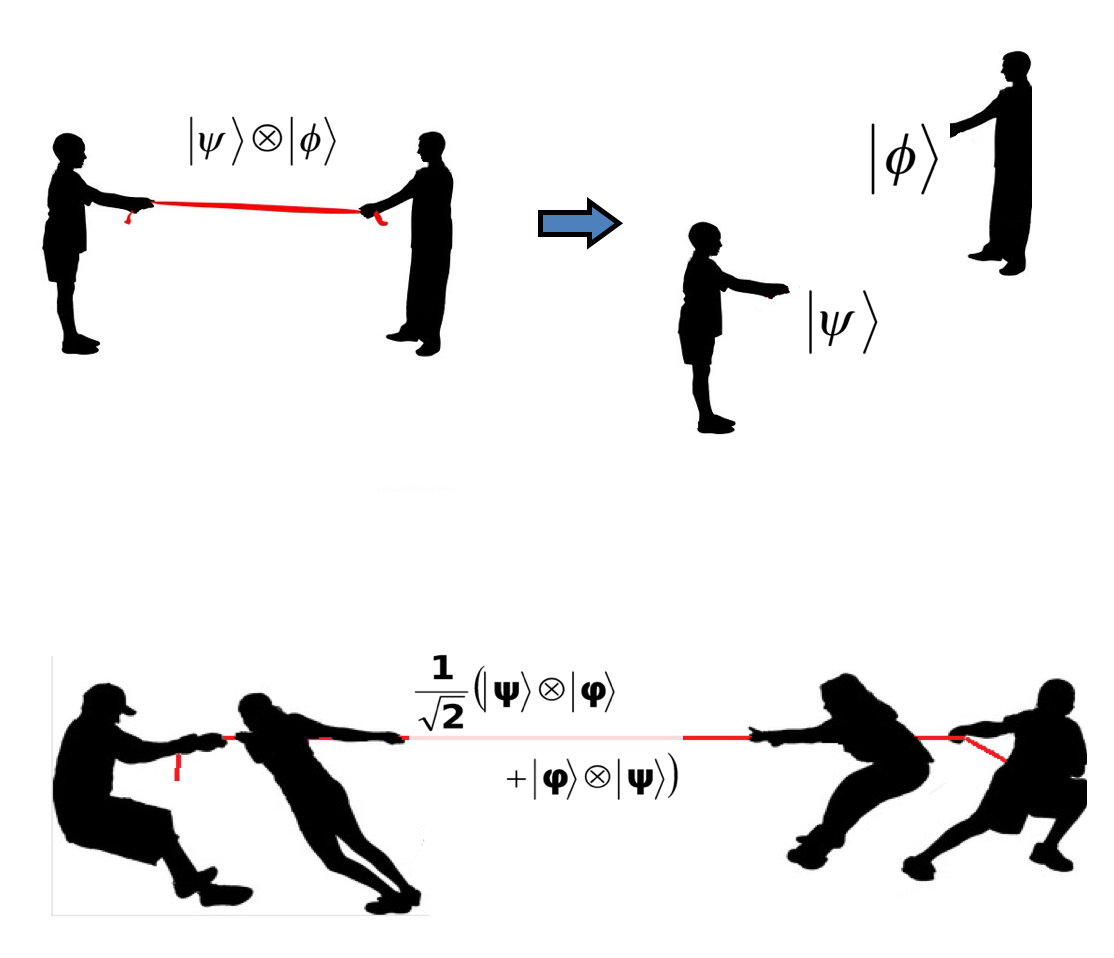
\includegraphics[width=\textwidth]{bi-entanglement.png}
   \end{figure}

   \column{0.5\textwidth}
   \begin{block}{}
     Работа Эйнштейна—Подольского-Розена\footnote[frame]{A. Einstein, B. Podolsky, and N. Rosen \textit{Phys. Rev.} \textbf{47}, 777 (1935)}
     указывала на неполноту квантовой механики с помощью мысленного эксперимента,
     заключающегося в измерении параметров микрообъекта косвенным образом,
     без непосредственного воздействия на этот объект.
   \end{block}
   \begin{block}{}
      В 2008 году был проведен эксперимент\footnote[frame]{T. Scheidl et al. \textit{PNAS} \textbf{107}, 46, 19708-19713 (2010)},
      который подтвердил нелокальный\footnote[frame]{J.S. Bell \textit{Physics Physique Fizika} \textbf{1}, 195 (1964)}
      характер квантовой теории.
   \end{block}
 \end{columns}
\end{frame}
\note{
  Первой работой в контекте квантовых корреляций принято считать статью опубликованную группой авторов ЭПР в 35 году.
  В работе обсуждалось парадоксальное поведение квантовой теории.
  Было показано, что существуют такие состояния,
  которые остаются взаимосвязанными даже за пределами светового конуса.

  Таким образом возможно измерение параметров удаленных микрообъектов косвенным образом.

  Разумеется вокруг работы разгорелись споры.

  В 64 году Джон Стюарт Белл предложил эксперимент, результат
  которого однозначно определял возможность таких корреляций.

  В 70 году Джоном Клаузером и  Аленом Аспе независимо были проведены первые эксперименты,
  которые подтвердили нелокальный характер квантовой теории.

  В настоящее время признано, что запутанность является ключевой концепцией квантовой теории.

  % Первый эксперимент был проведен Джоном Клаузером в 1972 (википедия).
  % Второй первый эксперимент был проведен Аленом Аспе в 70е.
  % (Alain Aspect Phys. Rev. D 14, 1944 – Published 15 October 1976)
  % И затем было еще много экспериментов.

  % В 2010 году Джон Клаузер, Ален Аспе и Антон Цайлингер стали лауреатами премии Вольфа по физике «за фундаментальный концептуальный и экспериментальный вклад в основы квантовой физики, в частности за серию возрастающих по сложности проверок неравенств Белла (или расширенных версий этих неравенств) с использованием запутанных квантовых состояний»
}

\begin{frame}{Бинарная запутанность}
  \begin{columns}
    \column{0.57\textwidth}
    $$
      \left| \Psi \right\rangle
      = \frac{
        \left| \uparrow\uparrow \right\rangle +
        \left| \downarrow\downarrow \right\rangle
      }{\sqrt{2}}
    $$
    \begin{block}{Критерии запутанности}
      \begin{itemize}
        \item Энтропия фон-Неймана \\
          {\footnotesize C.H.Bennett et al. \textit{Phys. Rev. A} \textbf{54}, 3824 (1996)}
        \item Критерий Вуттерса \\
          {\footnotesize W.K. Wootters, \textit{Phys. Rev. Lett.} \textbf{80}, 2245 (1998)}
        \item Мера Шмидта \\
          {\footnotesize Eisert J. and Briegel H. J. \textit{Phys. Rev. A} \textbf{64}, 022306 (2001)}
        \item ...
      \end{itemize}
    \end{block}

    %\begin{example}
    %  Запутанность в нитрозильном комплексе железа (НКЖ)\footnote[frame]{S. M. Aldoshin, E. B. Feldman, and M. A. Yurishchev, \textit{JETP} \textbf{107}, 5, 804–811 (2008)}.
    %\end{example}

    \column{0.4\textwidth}
    %\vspace{-2mm}
    \begin{figure}
      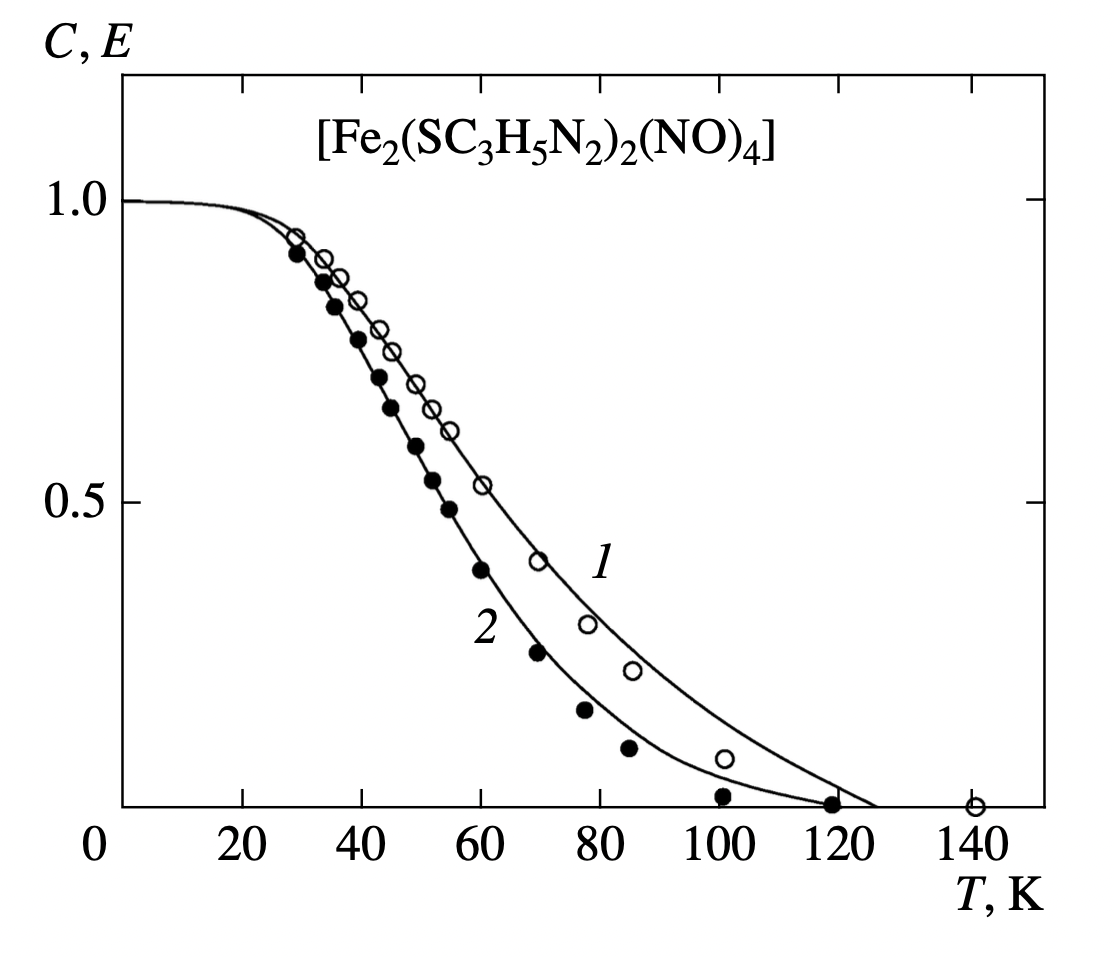
\includegraphics[width=\textwidth]{Aldoshin2008-concurence-by-temp.png}
      \captionsetup{skip=-2mm}
      \caption{Температурная зависимость согласованности (1) и запутанности (2) для нитрозильного комплекса железа\footnote[frame]{S. M. Aldoshin, E. B. Feldman, and M. A. Yurishchev, \textit{JETP} \textbf{107}, 5, 804–811 (2008)}.}
    \end{figure}
  \end{columns}
\end{frame}
\note{
  Определения таких состояний нетривиальная задача.
  В действительности, чтобы показать, что состояние запутанно нужно еще угадать с проективными измерениями,
  так как в произвольном базисе нельзя установить факт наличия запутанности.

  Эта задача уже хорошо разработана
  и было предложено множество критериев для выявления таких корреляций.
  например  мера Шмидта, согласованность Вуттерса, энропия фон-Неймана.


  Этот эффект хорошо изучен экспериментально, в качестве примера
  на слайде приведен результат из работы нашего института.
  Это температурная зависимость величины запутанности
  подсчитаной на основе согласованности в нитрозильном комплексе железа.
  Линии это теоретический расчет, точки это эксперимент.

  Такие результаты удается получит благодаря тому, ё
  что согласованность Вуттерса удалось связать с магнитной восприимчивостью атиферомагнитного димера.
}

\begin{frame}{Квантовые технологии}
  \begin{columns}
   \column{0.6\textwidth}
   \begin{figure}
     \begin{subfigure}[t]{0.33\textwidth}
       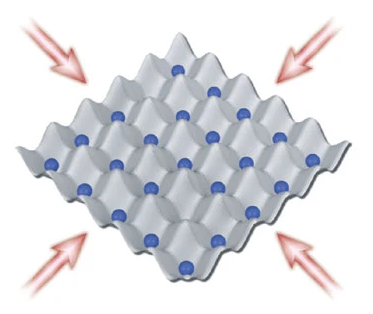
\includegraphics[width=\textwidth]{ultracold-atoms.png}
       %\captionsetup{labelformat=empty}
       \caption{Ultracold atoms}
       \label{fig:ultracold-atoms}
     \end{subfigure}
     \begin{subfigure}[t]{0.33\textwidth}
       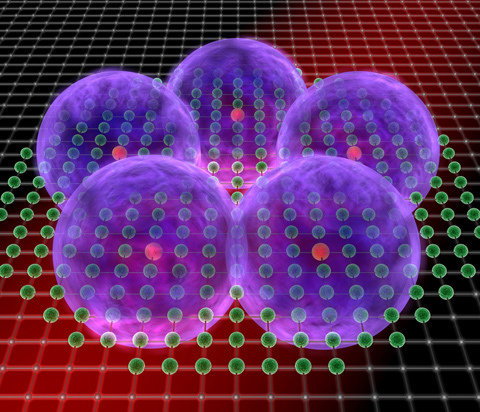
\includegraphics[width=\textwidth]{ridberg-atoms.png}
       %\captionsetup{labelformat=empty}
       \caption{Rydberg atoms}
     \end{subfigure}
     % \vspace*{2mm}
     \vfill
     \begin{subfigure}[t]{0.33\textwidth}
       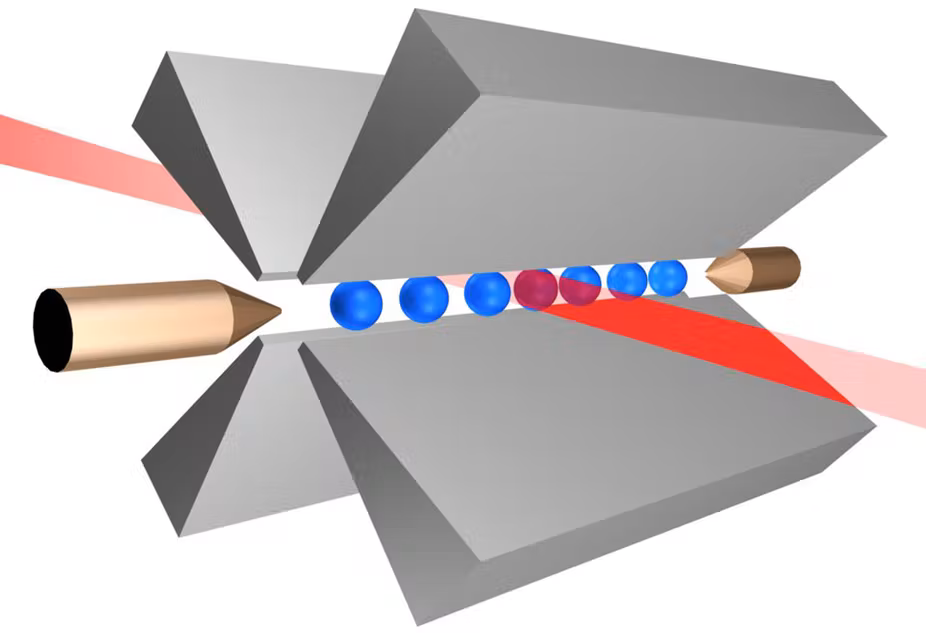
\includegraphics[width=\textwidth]{trapped-ions.png}
       %\captionsetup{labelformat=empty}
       \caption{Trapped ions}
     \end{subfigure}
     \begin{subfigure}[t]{0.33\textwidth}
       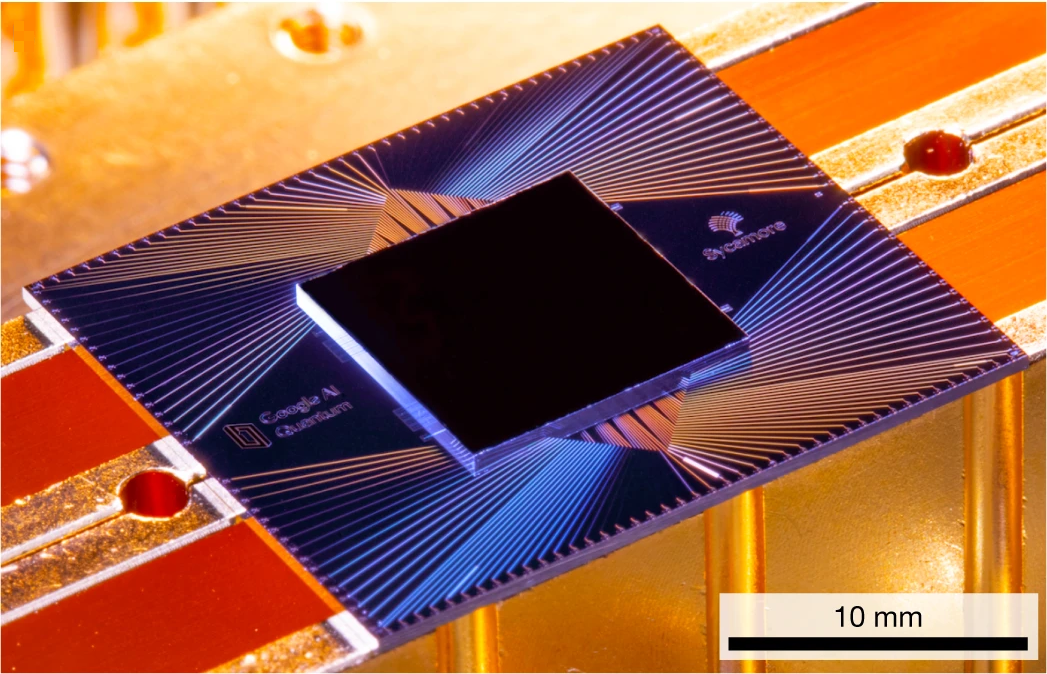
\includegraphics[width=\textwidth]{sycamore.png}
       %\captionsetup{labelformat=empty}
       \caption{SC qubits}
     \end{subfigure}
     \caption{
       Квантовые платформы.
       % (\ref{fig:ultracold-atoms})~{Bloch, I. Nature 453, 1016–1022 (2008)}
     }
   \end{figure}

   \column{0.4\textwidth}
   \begin{figure}
       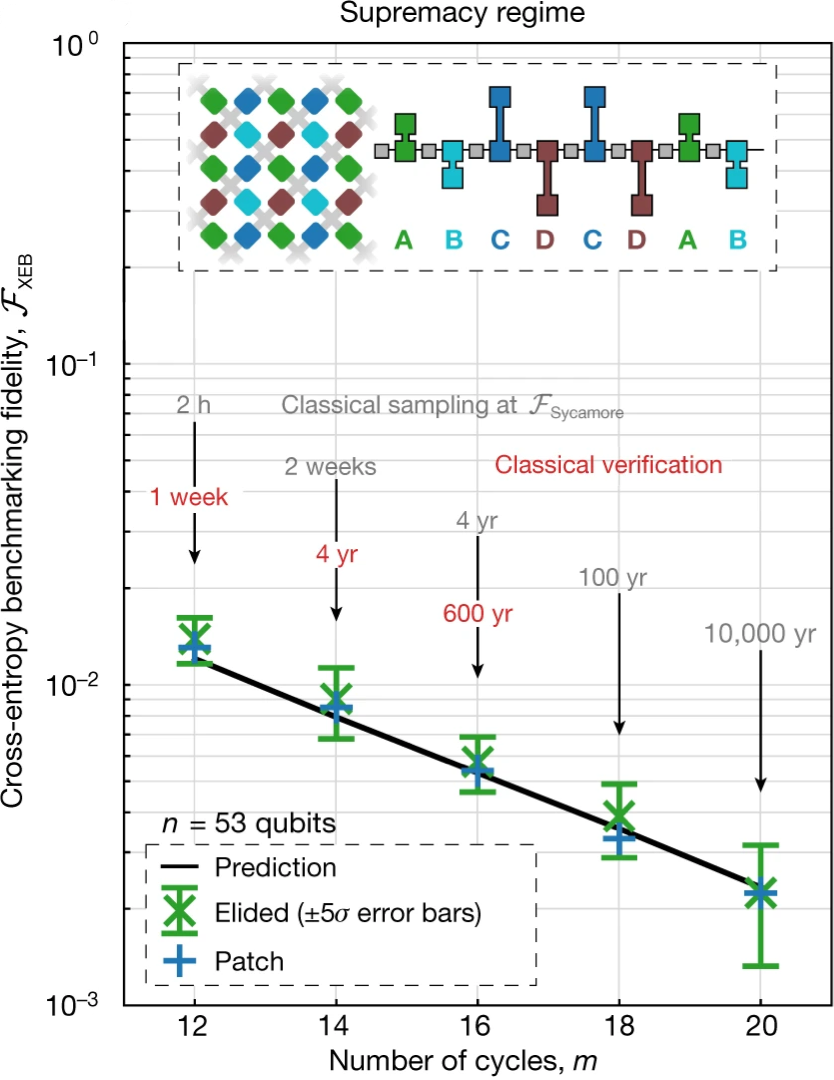
\includegraphics[width=0.8\textwidth]{sycamore-supemancy.png}
       % \captionsetup{labelformat=empty}
       \caption{
         % F. Arute et al., Nature 574, 505 (2019)
         Nature 574, 505 (2019)
       }
     \end{figure}
   \end{columns}
\end{frame}
\note{
  Тем неменее когда мы говорим о квантовом превосходстве
  мы иммеем ввиду большое количество взаимодействующих кубитов.
  Сейчас это порядка 50.
  Это значит, что главным реусурсом является не бинарная запутанность, а многокубитная.
  Предпринятые в данной работе попытки количественного определения запутанности мотивированы желанием понять и количественно оценить эти ресурсы.


  % \textbf{ЯМР}
  % ЯМР был первым, но он негодится для вычислений (нет чистых состояний).
  % Отлично подходит для исследований.
  % Много наработок.
%
  % Исследуется все гильбертого пространство.
  % Квантовое превосходство  на программируемом сверхпроводящем процессоре.
  % Запутанные состояния являются важным ресурсом в квантовых вычисления:
  % Например, недавно продемонстрированное группой Мартинеса квантовое превосходство [1] на программируемом сверхпроводящем процессоре связано с понятием запутанноси
}


\begin{frame}{Цели и задачи}
  \textbf{Целью данной работы} является теоретическое исследование многочастичной запутанности в системах с большим количеством частиц $(>200)$ в рамках МК спектроскопии ЯМР,
а также развитие методов экспериментального измерения величин квантовой информации Фишера и косой информации Вигнера-Янасе.
\end{frame}
\note{
  Целью данной работы является теоретическое исследование многочастичной запутанности в системах с большим количеством частиц.
  Так как мы хотим исследовать действительно большие системы,
  то наиболее удобным вариантом является твердотельный ЯМР.

  Как будет показано ниже, определение количества запуттаных спинов,
  это частный случай более сложной фундаментальной проблемы,
  а конкретно измерения квантовых информационных величин.
  Поэтому более общая цель работы это развитие экспериментальных методов измерения квантовой информации Фишера и косой информации.
}

\begin{frame}{Положения, выносимые на защиту}
  \begin{enumerate}
  \item 
  Разработана теория МК ЯМР для системы эквивалентных спинов при произвольной температуре.
  
  \item 
  Исследована температурная зависимость многочастичной запутанности в нанопоре, 
  когда система приготовлена в термодинамическом равновесном зеемановском и дипольно упорядоченном состояниях.
  
  \item
  Исследована многочастичная запутанность в квазиодномерных цепочках ядерных спинов в зависимости от параметров цепи и температуры.
  
  \item 
  Предложен метод экспериментального измерения точного значения косой информации Вигнера-Янасе в рамках МК спектроскопии ЯМР.
  
  \item 
  Проведено сравнение оценок многочастичной запутанности, полученных на основе квантовой информации Фишера и косой информации Вигнера-Янасе.
\end{enumerate}
\end{frame}
\note{
    Проведенные исследования позволяют заключить,
    что МК-спектроскопия ЯМР является тонким и полезным методом для исследования различных проблем квантовой информатики.
    В частности, это очень эффективный метод исследования квантовой запутанности.
}

\begin{frame}{Научная новизна и практическая ценность}
  \begin{block}{Научная новизна.}
    В данной работе была разработана теория МК ЯМР для нанопоры при произвольной температуре,
что позволило впервые теоретически исследовать температурную зависимость многочастичной запутанности в системе из более чем 200 взаимодействующих частиц.
Также в данной работе был разработан метод определения величины косой информации Вигнера-Янасе в МК эксперименте ЯМР.
  \end{block}

  \begin{block}{Практическая ценность.}
   Так как косая информация Вигнера-Янасе нашла много применений в квантовой теории информации, %~\cite{Wigner1963, Luo2017},
предлагаемый в данной работе метод определения ее величины
не только позволяет исследовать многочастичную запутанность методами МК ЯМР,
но и открывает возможность решения широкого класса задач в этой области.
  \end{block}
\end{frame}


\section{Исследование квантовых корреляции методами ЯМР}

\subsection{Многочастичная запутанность}
\begin{frame}{Многочастичная запутанность}
  $$
  \left| \Psi_{3-\mathrm{ent}} \right\rangle
  = \frac{1}{\sqrt{8}}
  \left| \uparrow_1 \right\rangle
  \otimes
  \left(
    \left| \uparrow_2\uparrow_4\right\rangle +
    \left|\downarrow_2\downarrow_4\right\rangle
  \right)
  \otimes
  \left(
    \left|\uparrow_3\uparrow_5\uparrow_9\right\rangle +
    \left|\downarrow_3\downarrow_5\downarrow_9\right\rangle
  \right)
  \otimes
  \left(
    \left|\uparrow_6\uparrow_7\uparrow_8\right\rangle +
    \left|\downarrow_6\downarrow_7\downarrow_8\right\rangle
  \right)
  $$
  \begin{alertblock}{Многочастичная запутанность $k$-частиц}
  $$
  \left| \Psi_{k-\mathrm{ent}} \right\rangle
  	= \otimes^\mathrm{M}_{i=1} \left| \Psi_{i} \right\rangle,
  $$
  где $\left| \Psi_{i} \right\rangle$ это состояние подсистемы с $N_i$ частиц,
  $ \sum\limits_{i=1}^N N_i = N $
  и $ \exists m: N_{m} \ge k$
  \end{alertblock}

\end{frame}
\note{
  А вот многочастичная запутанность изучена гораздо хуже,
  так как для этого нужно исследовать многочастичные системы,
  пространство которой экспоненциально растет с увеличение числа частиц.

  Также не очевидно какое определение должнобыть у многочастичной запутанности.

  В нашей работе мы используем для многочастичной запутанности  следующее определение: ...слайд...

  То есть наличие запутанности порядка $k$,
  говорит о том что существует несепарабельная подсистема размера $k$.
}

\begin{frame}{Меры многочастичной запутанности}
  \vspace{-2mm}
  \begin{block}{Свойства}
    \begin{enumerate}
      \item $
        F(\rho_1 \otimes \rho_2 ,H_1 \otimes I_2 + I_1 \otimes H_2)
    	= F_{1} (\rho_1, H_1) + F_{2} (\rho_2 , H_2)
      $
      \item $F \leq N^2$
    \end{enumerate}
  \end{block}
  \vspace{-1mm}
  \begin{alertblock}{Нижняя граница числа запутанных спинов}
    Пусть в системе максимальный размер несепарабельной подсистемы равен $k$, тогда
    $$ F^{k} \leq \left[ \frac N k \right] k^2 + \left(N - k \left[ \frac N k \right]\right)^2 $$
  \end{alertblock}
  \vspace{-1mm}
  \begin{examples}
    \begin{enumerate}
      \item Косая информация Вигнера-Янасе\footnote[frame]{Zeqian Chen \textit{Phys. Rev. A} \textbf{71}, 052302 (2005)}
      \item Квантовая информация Фишера\footnote[frame]{P. Hyllus et al. \textit{Phys. Rev. A} \textbf{85}, 022321 (2012)}
    \end{enumerate}
  \end{examples}
\end{frame}
\note{

Нас интересует два свойства меры:
1. В сепарабельной системе с матрицей плотности $\rho = \rho_1 \otimes \rho_2$ квантовая информация Фишера удовлетворяет условию аддитивности)
2. Известна ее верхняя граница $F_\mathrm{Q} \leq N^2$, где $N$ это количество частиц в системе.

Благодаря этим свойствам, зная величину меры в системе можем оценить нижнюю границу количества запутанных частиц в системе. То есть если в системе максимальный размер не сепарабельной подистемы равен $k$, то
мера такой всей системы точно не больше данного значеничя: ...слайд...

Таким образом получив значение меры  выше при фиксированом $k$ ...слайд...,  мы можем утверждать что существует несепарабельная системы размера больше $k$ расчитать дать нижнюю оценку на минимальный размер несепарпбельной системы.

Какие величины имееют такие свойства?
В квантовой теории информации есть ...слайд...
Эти величины сами по себе очень интересные.
}


\begin{frame}{Меры многочастичной запутанности}

Фиксируем какое-то значение $k$ - максимальное количество спинов в несепарабельной подсистеме
$$ N > k \geq N_1 \geq N_2 \geq \dots \geq N_l, \quad \sum_{i=0}^{l} N_i = N, $$
где $l$ количество несепарабельных подсистем.

Верхняя граница информации Фишера для такой системы:
$$
F^k = F_{1} + \dots + F_{l}
\leq N^2_1 + \dots + N^2_e
\leq \underbrace{
	k^2 + k^2 + \dots + k^2
	}_{m = \left[\frac N k \right] \, \mbox{раз}}
	+ \underbrace{(N-km)^2}_{\mbox{остаток}}
$$

\begin{alertblock}{}
    $$  F^k \leq \left[ \frac N k \right] k^2 + \left(N - k \left[ \frac N k \right]\right)^2 $$
\end{alertblock}
\end{frame}
\note{
Доказательства этого факта сводится к вычислению верхней границы квантовой информации Фишера для с фиксированым размером не сепарабельных подсистем.
Мы для себя фиксируем какое-то значение $k$ - максимальное количество спинов в несепарабельной подсистеме. Сделаем оценку сверху для информации Фишера.

Пусть есть я ...

Рассмотрим пару подсистем для которых верно $k > N_i > N_{i-1} > 0$.
Квантовая информации Фишера этих двух подсистем:
$$
F_{Q\,i,i-1} \leq N_{i}^2 + N_{i-1}^2
$$
При этом если мы рассмотрим случай когда в правой системе на один спин меньше, а в левой на одим больше то оценка верхней границы будет выше:
$$
\bar F_{Q\,i,i-1}
	\leq \left( N_{i}^2 + 1 \right)
		+ \left( N_{i-1}^2 - 1\right)
	\leq N_{i}^2 + N_{i-1}^2
		+ 2 \left(N_{i} - N_{i-1} + 1 \right)
$$
Следовательно в худшем случае...???

Следовательно если мы подсчитаем информацию Фишера, то мы
можем дать нижнюю границу количества запутанных частиц.
}

\subsection{Квантовая информация Фишера}
\begin{frame}{Квантовая информация Фишера}
  \begin{block}{}
    Квантовая информация Фишера\footnote[frame]{D. Petz and C. I Ghinea, \textit{Quantum Probab. Relat. Top.} (2011)}
    показывает,
    как быстро изменяется квантовое состояние,
    определяемое матрицей плотности,
    при изменении некоторого параметра.
  \end{block}
  Квантовая информация Фишера --- это прямой аналог классической информации Фишера и основная мера в квантовой метрологии.
  Квантовая информация Фишера $F_Q$ для матрицы плотности $\rho$ по отношению к наблюдаемой $A$:
  $$
    F_Q \left(\rho, A \right) =
      2\sum_{j,k} \frac{\left(\lambda_j - \lambda_k \right)^2}
        {\lambda_j + \lambda_k}
      \left| \langle j|A|k \rangle \right|^2,
  $$
  где $\lambda_k$ и $|k \rangle$ --- собственное значение и собственный вектор матрицы плотности $\rho$.
\end{frame}
\note{
Определение: Квантовая информация Фишера [qfi](QFI) показывает, как быстро из- меняется квантовое состояние, определяемое матрицей плотности, при изменении некоторого параметра. Как правило этот параметр является временем эволюции квантового состояния.
}

\subsection{Косая информация Вигнера-Янасе}
\begin{frame}{Косая информация Вигнера-Янасе}
  \begin{block}{}
    Косая информация\footnote[frame]{
      E. P. Wigner and M. M. Yanase,
      \textit{Proc. Nat. Acad. Sci. USA},
      \textbf{49}, 910–918 (1963)
    }
    была введена Вигнером и Янасе в контексте квантовых измерении в качестве меры информации,
    содержащейся в векторе квантового состояния, лежащего под углом по отношению к наблюдаемой $A$.
  \end{block}
  $$
    I_{WY}(\rho, A)
    = -\frac{1}{2} Tr([\sqrt{\rho}, A])^2
    = Tr(\rho A^2) - Tr(\sqrt \rho A \sqrt \rho  A )
  $$
  Для чистых состояний:
  $$
    I_{WY}(| \psi \rangle, A)
    = \langle \psi | A^2 | \psi \rangle - \langle \psi | A| \psi \rangle ^2
  $$
  \vspace{-5mm}
  \begin{block}{}
    Можно интерпретировать\footnote[frame]{S. Luo, \textit{Phys. Rev. Lett.} \textbf{91}, 180403 (2003)},
    косую информацию
    как квантовая неопределенность наблюдаемой $A$ для квантового состояния $\rho$.
  \end{block}
\end{frame}
\note{
    Косая информация была введена Вигнером и Янасе в контексте квантовых измерении.
    Позднее было признано, что косая информация,
    помимо своего изначального значения как меры информационного содержания состояний,
    допускает также несколько интерпретаций,
    носящих более физический и теоретико-информационный характер.

    В настоящее время эта величина нашла много применений в квантовой информации.

    Интригующей и тонкой особенностью косой информации является использование в ней квадратного корня из вектора квантового состояния (оператора плотности).

    Но тут

    % Skew information was introduced by Wigner and Yanase in the context of quantum measurements.
    % It is the quantity as a measure of the information content of the quantum state $\rho$ \textit{skew} to the observable $H$.
    % Here, \textit{tr} denotes the operator trace, and brackets denotes the commutator between operators.
%
    % Not that skew information is quite different from, but deeply related to, the ubiquitous von Neumann entropy [1]–[4].
    % Alse from a dual standpoint, we can interpret skew information
    % as the quantum uncertainty of the observable $A$ in the quantum state $\rho$ [5]–[8].
%
    % Skew information has many nice properties and interpretations that make it useful in quantum information theory[1], [8].
    % For example, skew information can be used to construct measures of quantum correlations [9]–[11],
    % to quantify quantum coherence [12]–[15], to quantify asymmetry [15], and so on.
    % It has also been used to study quantum phase transitions [16]–[20], uncertainty relations [6], [21]–[23], et cetera.
%
    % However such investigations like many-particle entanglement require the development of corresponding experimental methods.
    % In particular, it was shown [6] that a lower bound on the quantum Fisher information coincides with the double
    % second moment of the spectrum of multiple quantum (MQ) coherences.
    % % M. G\"arttner, P. Hauke, and A.M. Rey.Phys. Rev.Lett. 120, 040402, 2018
%
    % Bellow we demonstrate that the Wigner–Yanase information in a spin system (s = 1/2) with the dipole–dipole interactions
    % (DDI) in the MQ NMR experiment also connected to second moment of the spectrum of multiple quantum
    % (MQ) coherences.
%
    % It is not a random magic because skew information may be identifier as a paradigmatic version of quantum Fisher information.
    % % the statistical idea underlying the skew information is the Fisher information in the theory
    % % of statistical estimation.
}%


\subsection{Многоквантовая спектроскопия ЯМР}
\begin{frame}{Многоквантовый эксперимент ЯМР\footnote[frame]{
J. Baum, M. Munowitz, A. N. Garroway, and A. Pines, J. Chem. Phys. 83, 2015 (1985).}}

  \begin{figure}
    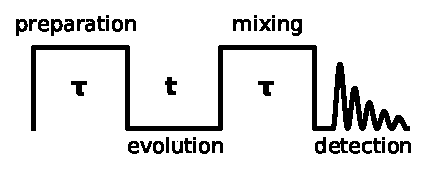
\includegraphics[width=0.5\textwidth]{mq-experiment-schema.pdf}
    %\caption{Схема МК эксперимента ЯМР}
  \end{figure}
  \vspace{-3mm}
  \begin{block}{}
    На подготовительном периоде МК эксперимента ЯМР система облучается последовательностью радиочастотных импульсов. В результате динамика спиновой системы определяется многоквантовым гамильтонианом.
    $$
    H_{MQ} = H^{(2)} + H^{(-2)},
    \quad H^{(\pm2)} = \frac 1 2 \sum_{i < j} D_{ij} I^\pm_i I^\pm_j
    $$
  \end{block}
\end{frame}
\note{
     МК динамику мы решили исследовать стандартным МК экспериментом.
     Эксперимент состоит из четырех частей,
     но нас будет интересовать только подготовительный период эксперимента.
     На подготовительном периоде ...слайд...
}

\begin{frame}{Многоквантовый экперимент ЯМР}
  \begin{columns}
    \column{0.4\textwidth}

    \begin{figure}
      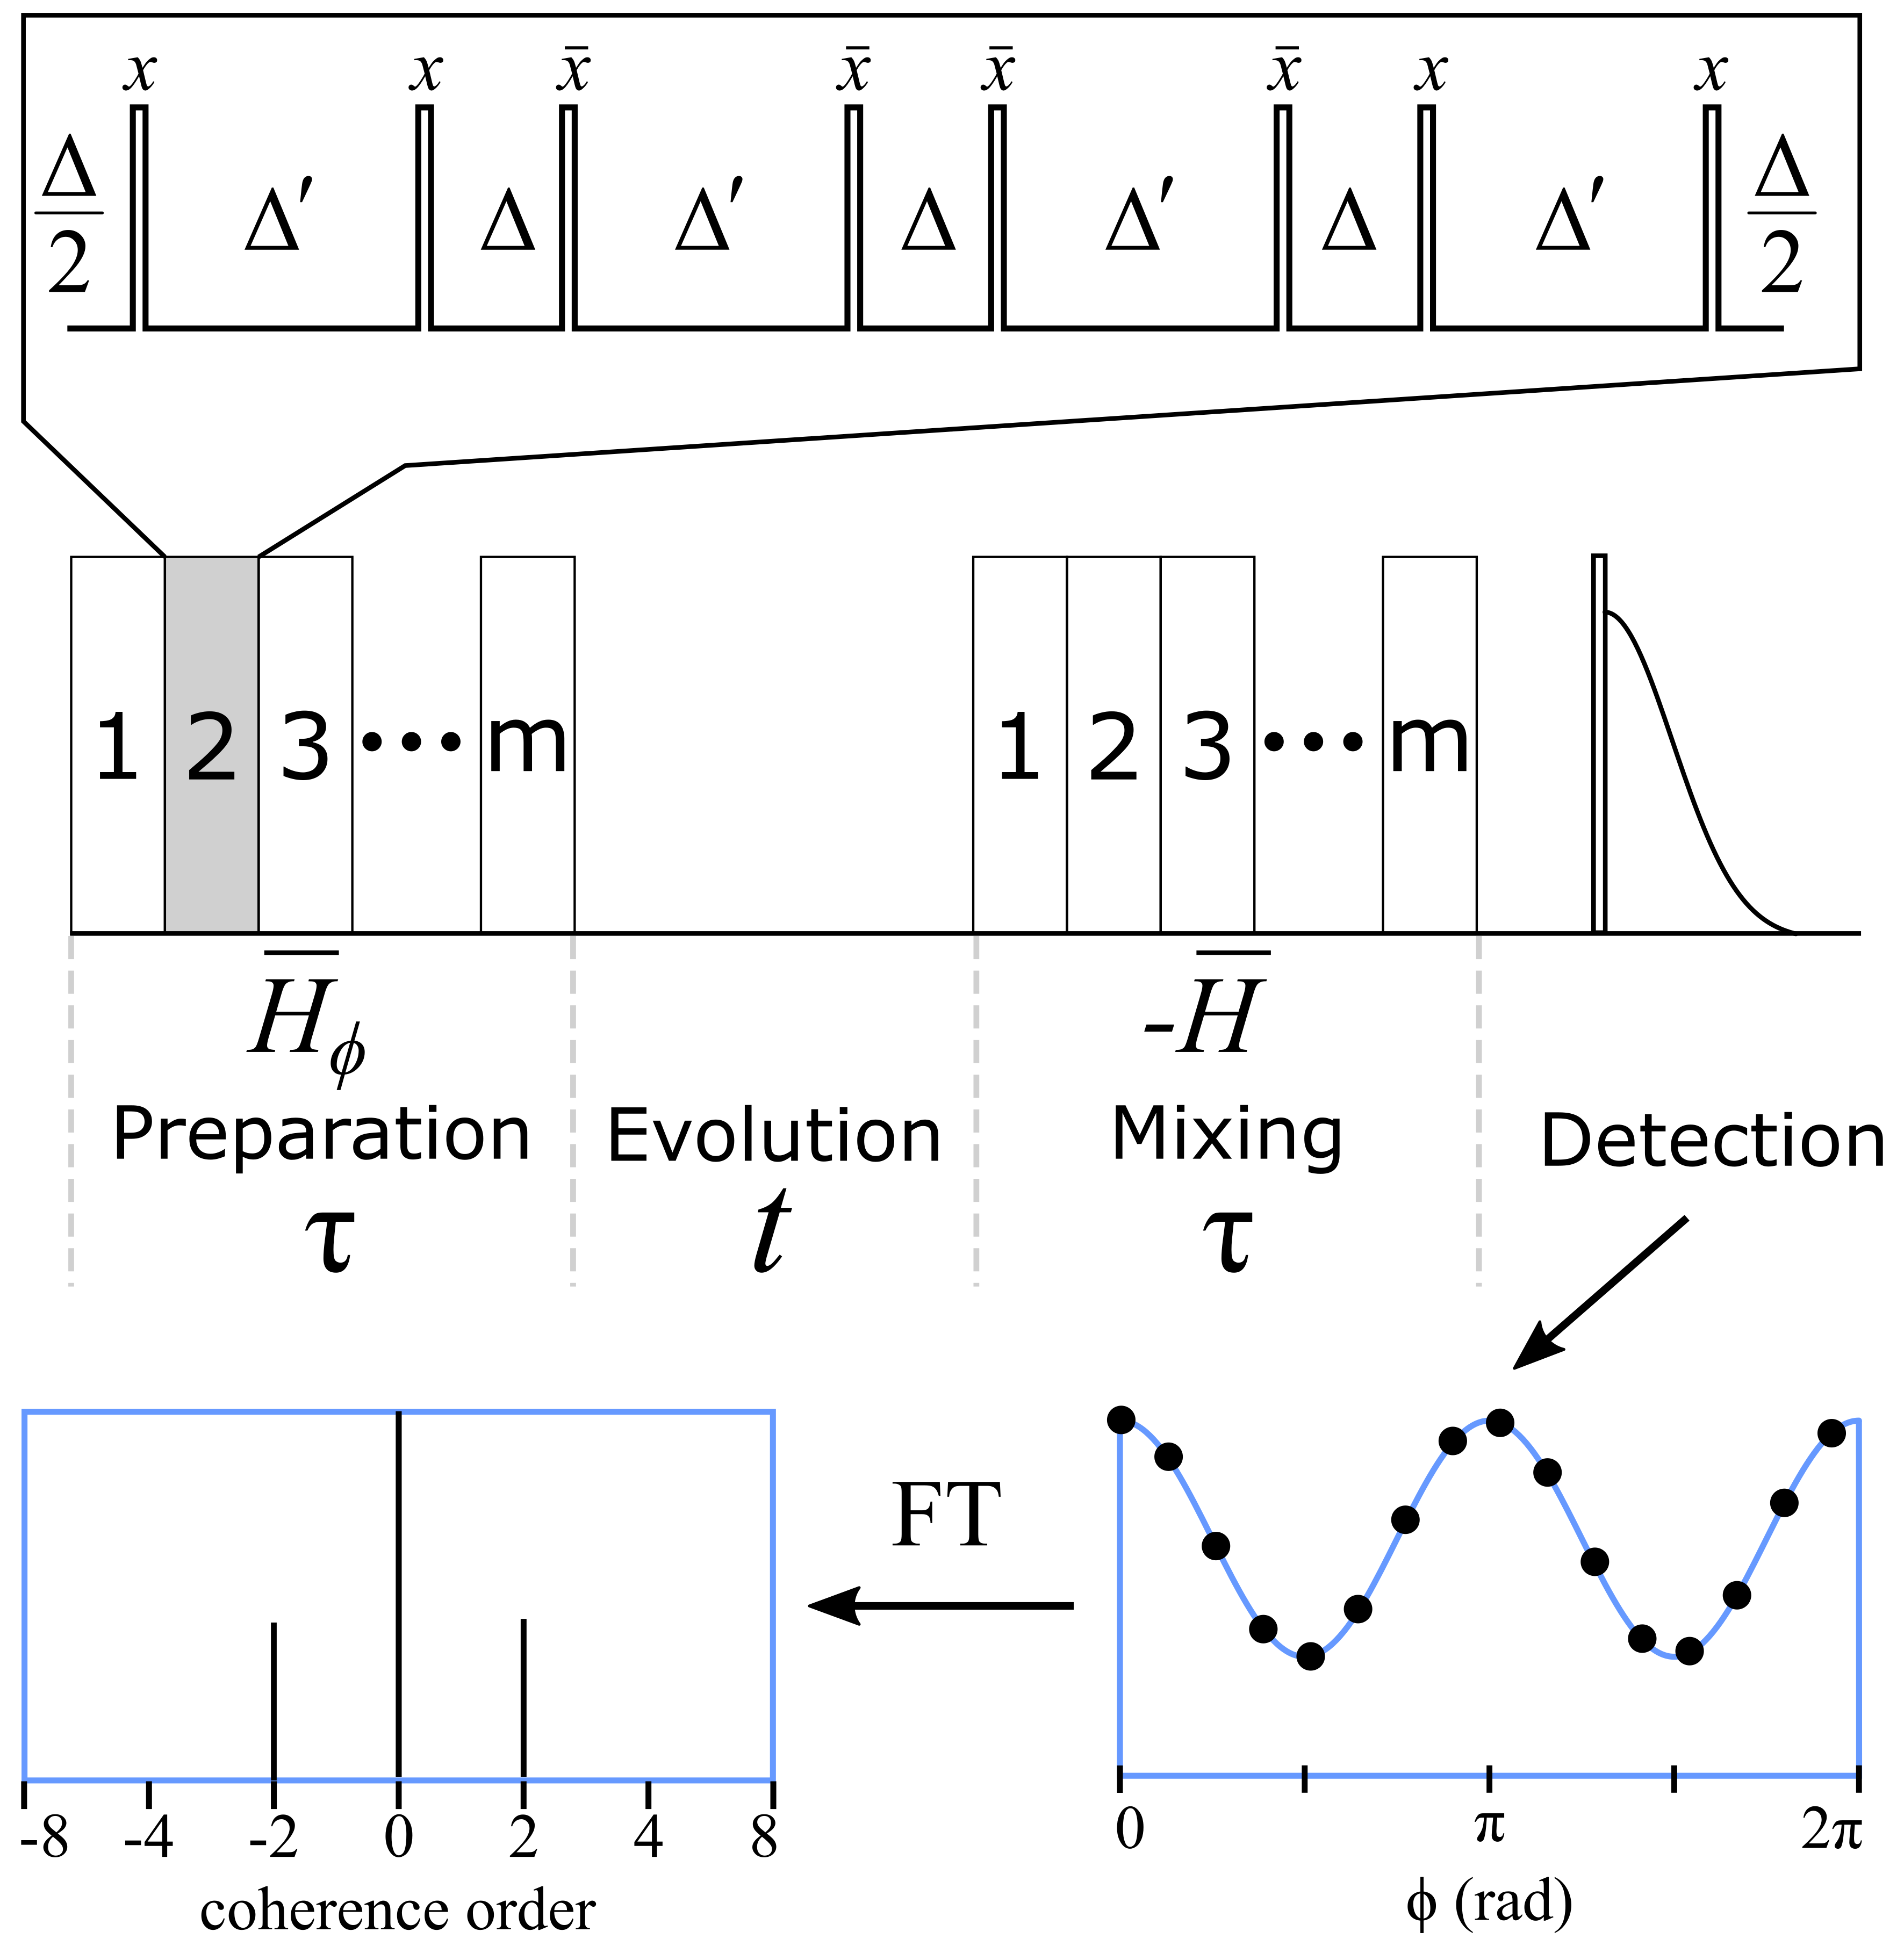
\includegraphics[width=0.9\textwidth]{mq-experiment-pulses-schema.png}
      \caption{Схематичное представление последовательности импульсов МК эксперимента.}
    \end{figure}


    \column{0.6\textwidth}
    МК когерентности создаются в течение периода подготовки продолжительностью $\tau$ при участии m-серии 8-импульсовых подпоследовательностей и затем преобразуются в наблюдаемую намагниченность после идентичного периода смешивания (за исключением 90-градусного фазового сдвига). Затем намагниченность детектируется при импульсе $\pi/2$. Фазовый сдвиг $\phi$ между периодами подготовки и смешивания инкриминируется для разделения многоквантовых когерентностей разных порядков. В результате преобразования Фурье по $\phi$ получается МК ЯМР спектр. Интенсивности МК когерентностей ЯМР при различных длительностях периода свободной эволюции $t$ получаются в отдельных экспериментах.
  \end{columns}
\end{frame}
\begin{frame}{Распределение интенсивности МК когерентностей ЯМР}
\begin{columns}
  \column{0.4\textwidth}
  \vspace{-3mm}
  \begin{figure}
    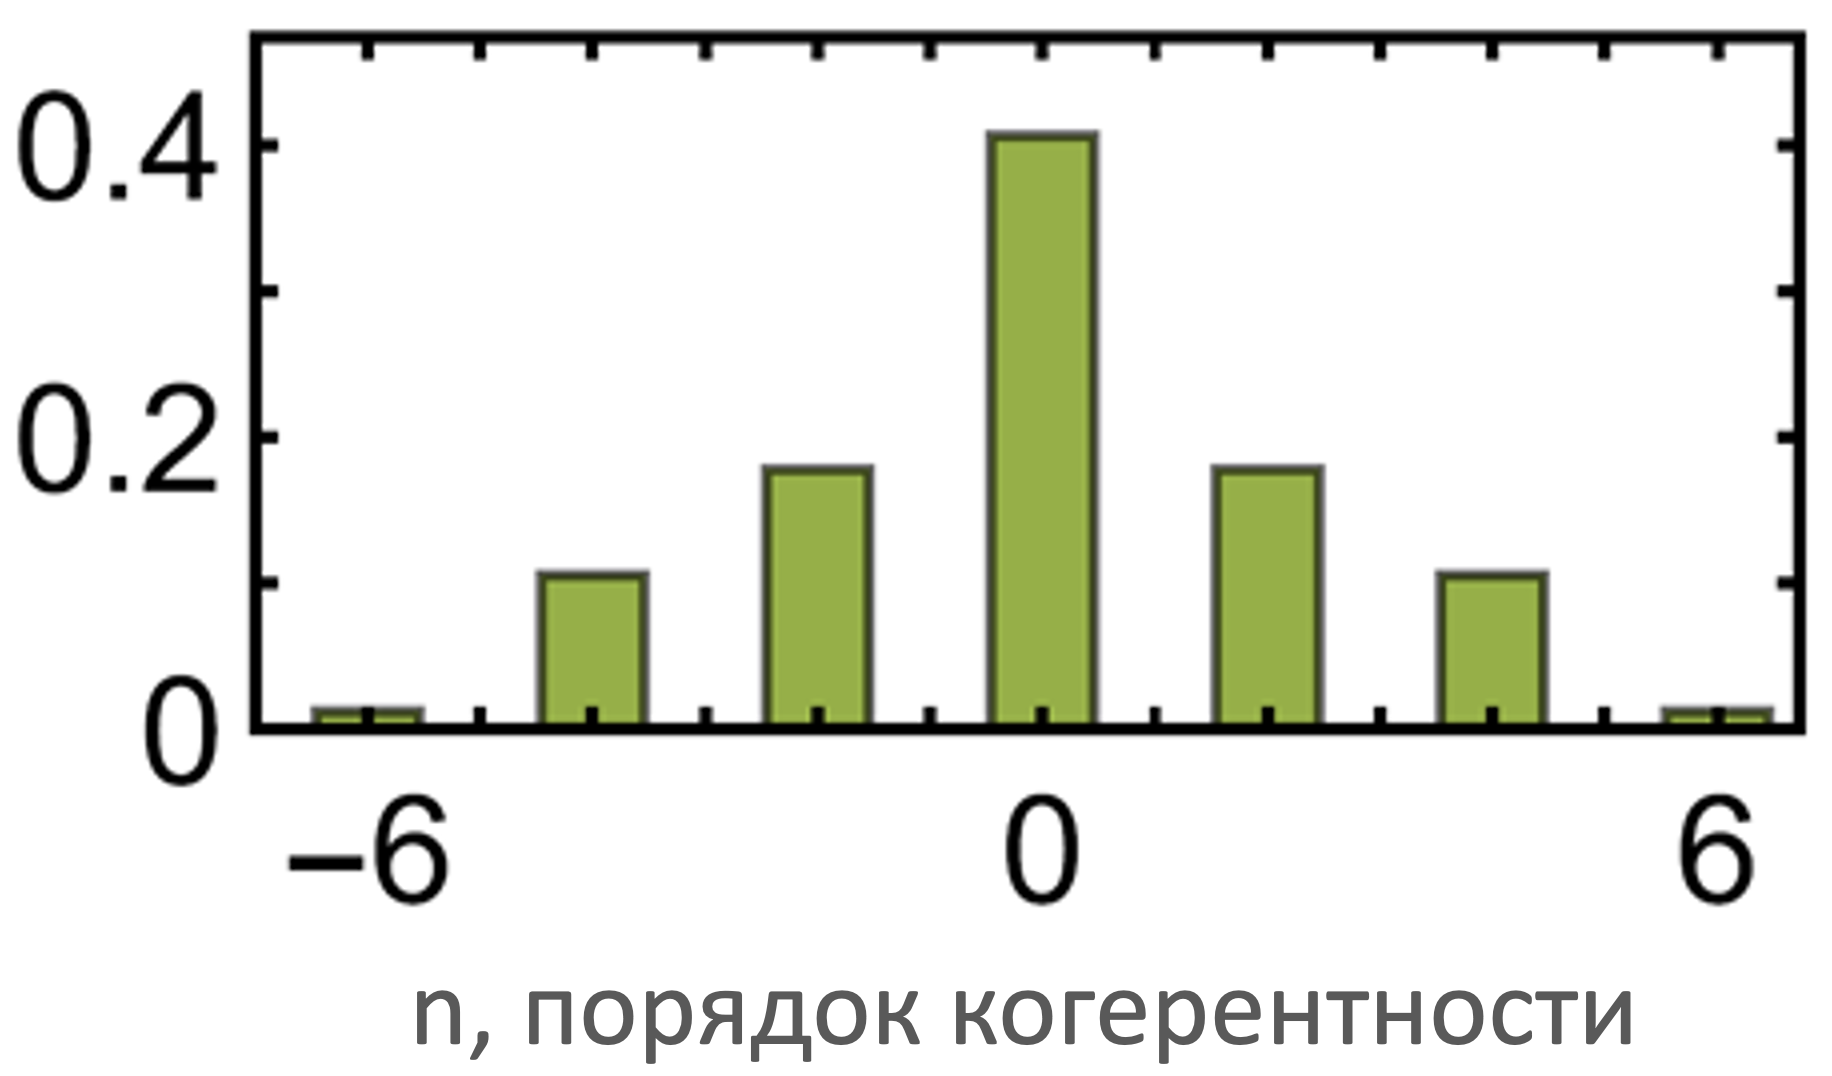
\includegraphics[width=\textwidth]{mq-coherence-intensities-hist.png}
    \caption{Распределение интенсивности МК когерентностей ЯМР.}
  \end{figure}

    \column{0.5\textwidth}
    \begin{block}{}
      Второй момент (дисперсия) распределения МК когерентностей ЯМР.
      $$
        M_2 (\tau,\beta) = \sum_n n^2 J_n(\tau,\beta)
      $$
      где $J_n$ интенсивность МК когерентности ЯМР порядка $n$.
    \end{block}

\end{columns}
\end{frame}
\note{
  Подсчитать информацию фишера не просто подсчитить но она связана с рейльной физической величеной.
  Важно отметить что здесь нам удалось связать меру информации с физической величиной.
  Под действием гамильтониана происходят переходы между энергетическими уровнями
  и возникаюм многоквантовые когерентности.
  Гистограма показывает частоту этих переходов.
  ЯМР отличный инструмент и наша работа это подтверждает.

  % mq-coherences-distribution % JETP 2018
}



\section{Измерение информации Фишера в МК эксперименте ЯМР}
\begin{frame}{Определение информации Фишера в МК ЯМР (PRA-19)\footnote{S.I. Doronin, E.B. Fel'dman,  I.D. Lazarev, \textit{Phys. Rev. A}, \textbf{100}, 022330 (2019)}}
  $$ G(\tau, \phi) =
     \mathrm{Tr}\left\{
         e^{iH_\mathrm{MQ}\tau} e^{i\phi I_z} e^{-iH_\mathrm{MQ}\tau}
         \rho_\mathrm{eq}
         e^{iH_\mathrm{MQ}\tau} e^{-i\phi I_z} e^{-iH_\mathrm{MQ}\tau}
         I_z \right\}
  $$
  \begin{alertblock}{}
      Дисперсия распределения интенсивности МК когерентностей ЯМР определяет нижнюю границу информации
      Фишера\footnote[frame]{
      M. G\"arttner, P. Hauke, and A.M. Rey. \textit{Phys. Rev. Lett.} \textbf{120}, 040402 (2018)}:
      $$
      F_Q \geq 2M_2
      $$
  \end{alertblock}
  Однако формула справедлива только в том случае,
  если сигнал $G(\tau, \varphi)$ является \textit{out-of-time-ordered correlator} (OTOC).
  Для низких температур это условие не выполняется.
  Возможно обойти это ограничение,
  если усреднить сигнал МК эксперимента ЯМР по начальному состоянию:
  $$ G_\mathrm{LT}(\tau, \phi)
     = \mathrm{Tr}\left\{
       e^{iH_\mathrm{MQ}\tau} e^{i\phi I_z} e^{-iH_\mathrm{MQ}\tau}
       \rho_\mathrm{eq}
       e^{iH_\mathrm{MQ}\tau} e^{-i\phi I_z} e^{-iH_\mathrm{MQ}\tau}
       {\color{red} \rho_\mathrm{eq}}
    \right\}
  $$
\end{frame}




\section{Многочастичная запутанность в системе эквивалентных спинов}
\begin{frame}{Система эквивалентных спинов}
  \begin{figure}
    \begin{subfigure}[t]{0.32\textwidth}
      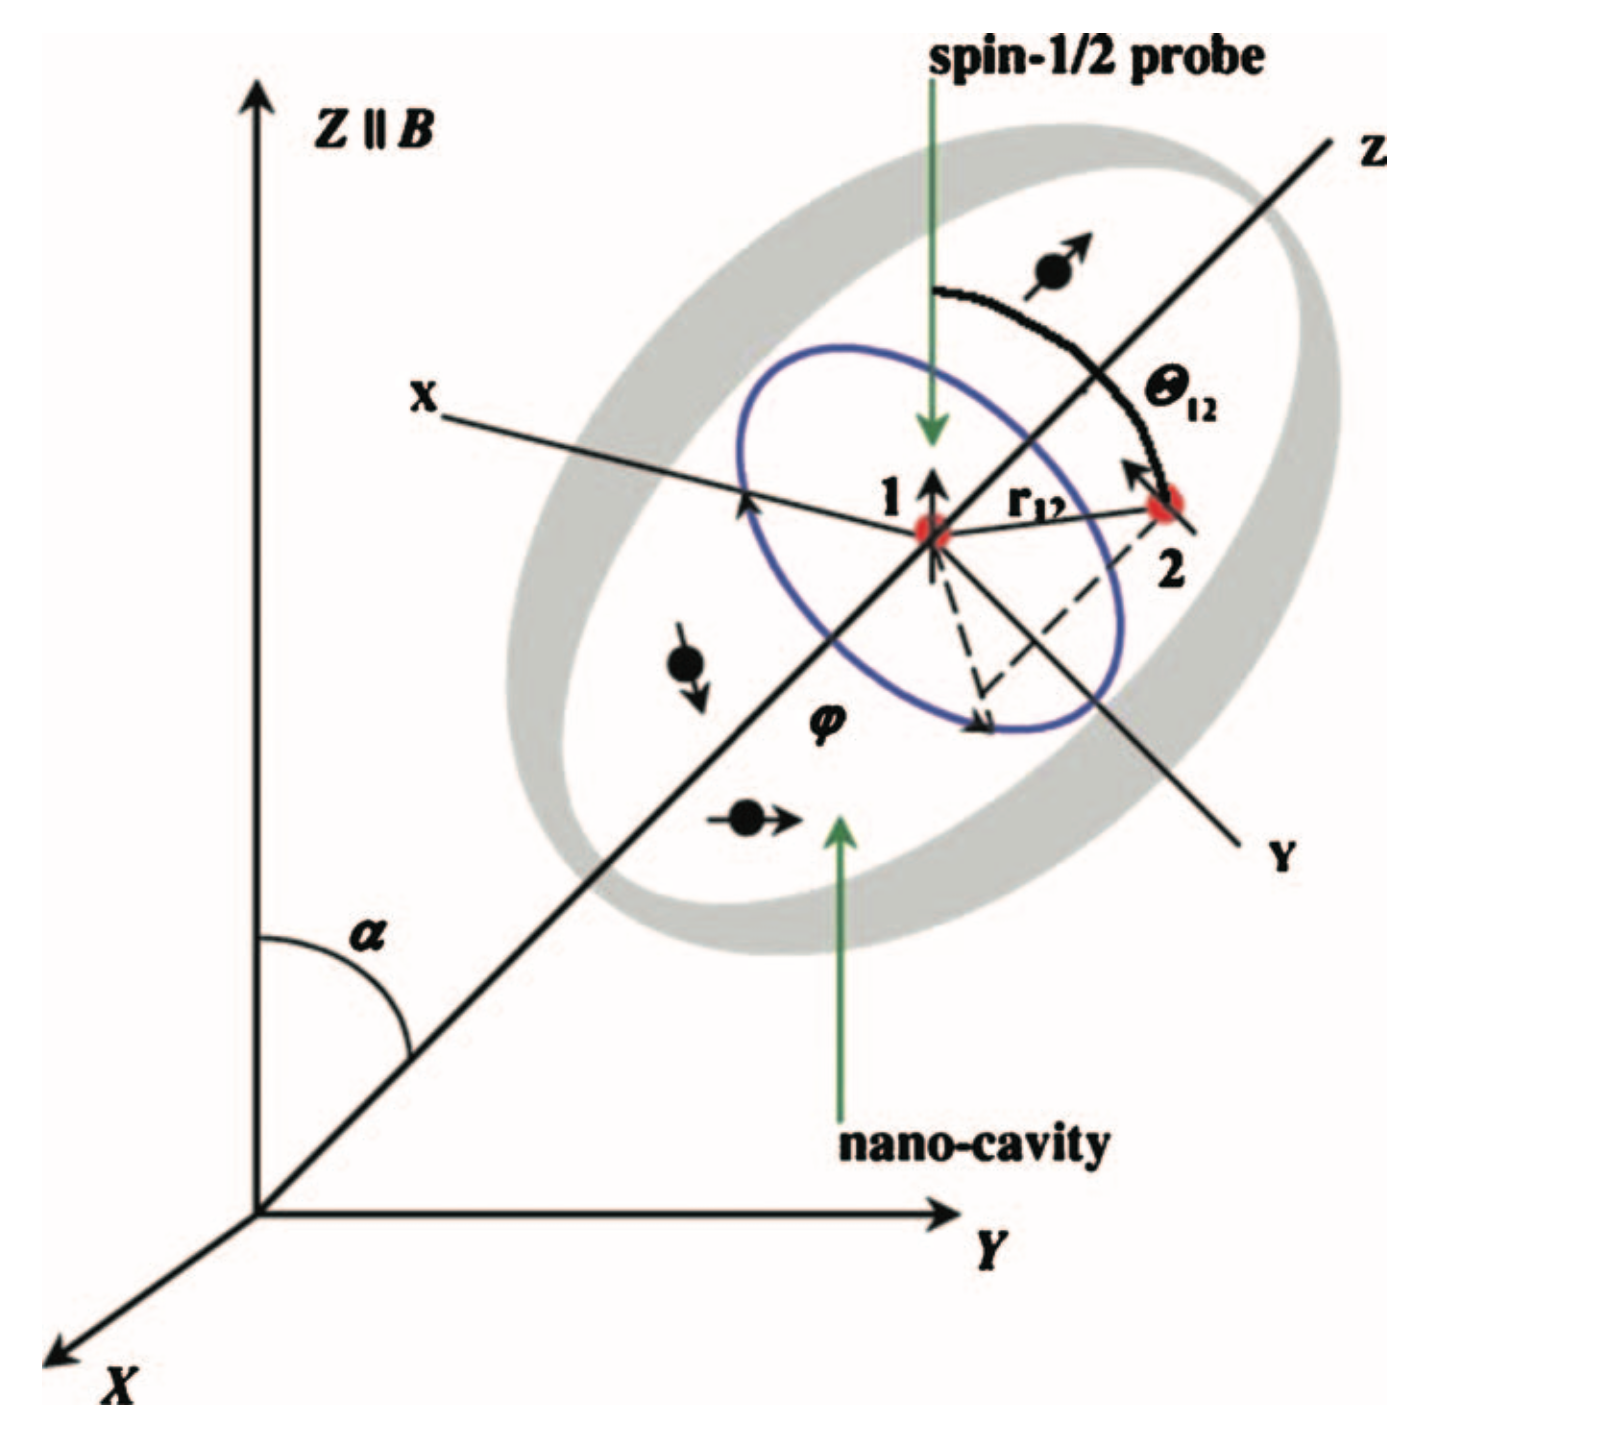
\includegraphics[width=\textwidth]{model-nanopore-schema.png}
      \caption{
        Hанопора\footnote[frame]{J. Baugh, A. Kleinhammes, D. Han, Q. Wang, and Y. Wu, \textit{Science} \textbf{294}, 1505 (2001).}
        со спин-несущих молекулами во внешнем сильном магнитном поле $\vec B$.
      }
    \end{subfigure}
    \hfill
    \begin{subfigure}[t]{0.32\textwidth}
      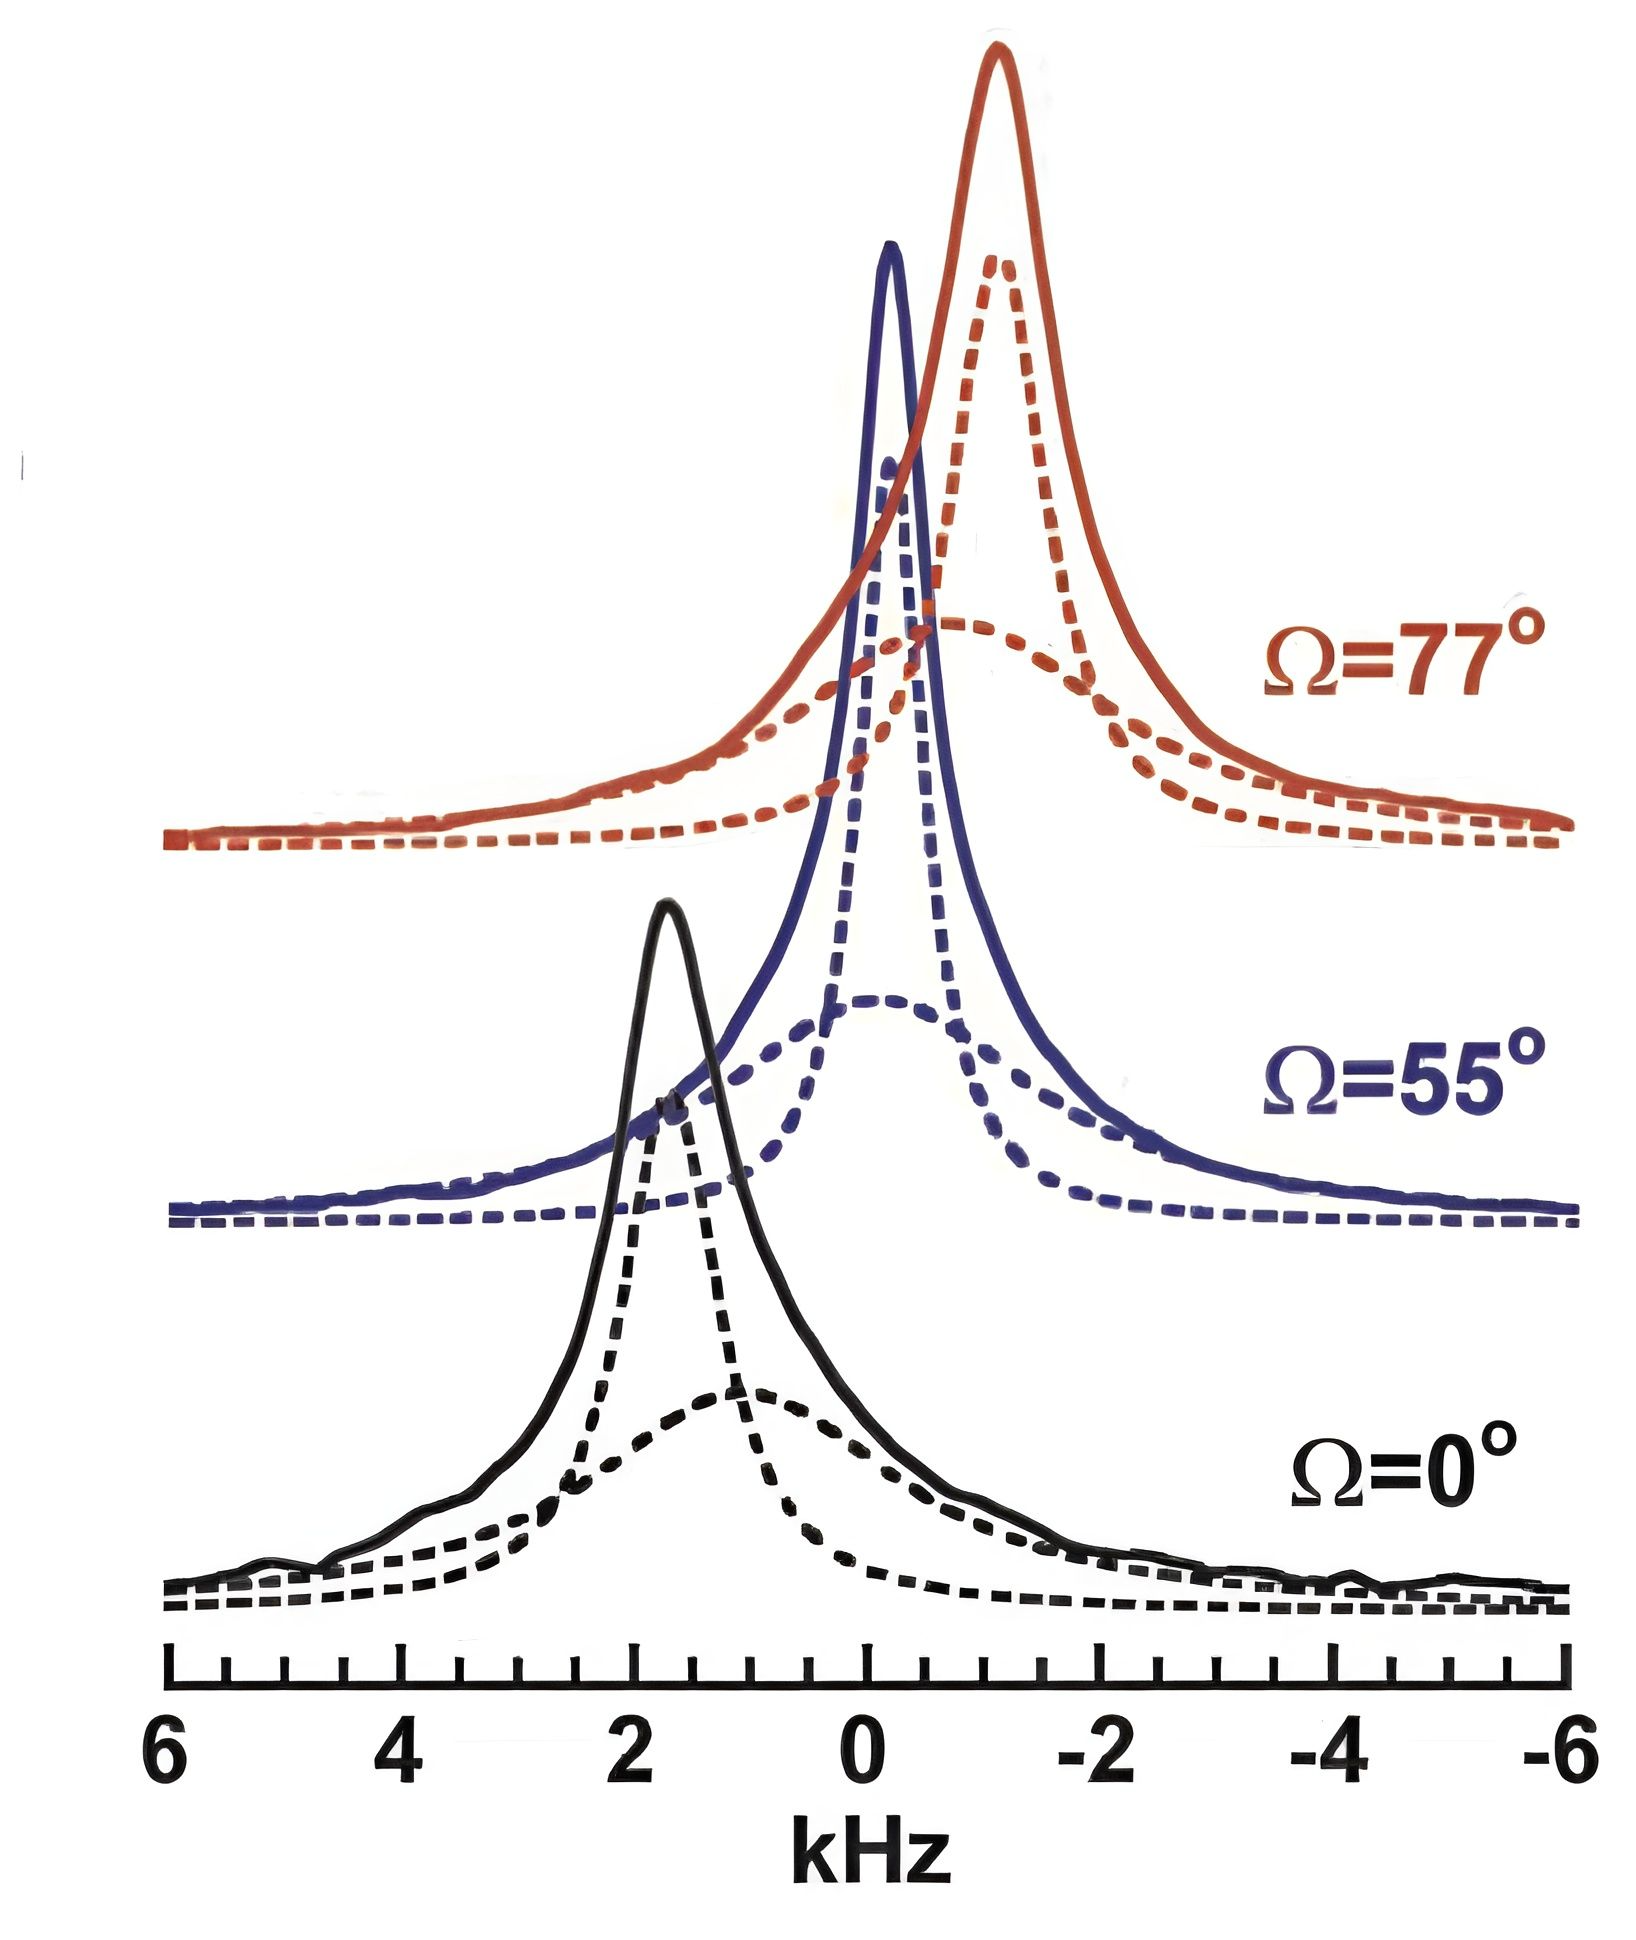
\includegraphics[width=0.8\textwidth]{sample-nanopore-nmr-spectrum.png}
      \caption{
        Молекулярная диффузия газа быстрее флип-флоп процессов.
        Вся система характеризуется одной константой $D$.
      }
    \end{subfigure}
    \hfill
    \begin{subfigure}[t]{0.32\textwidth}
      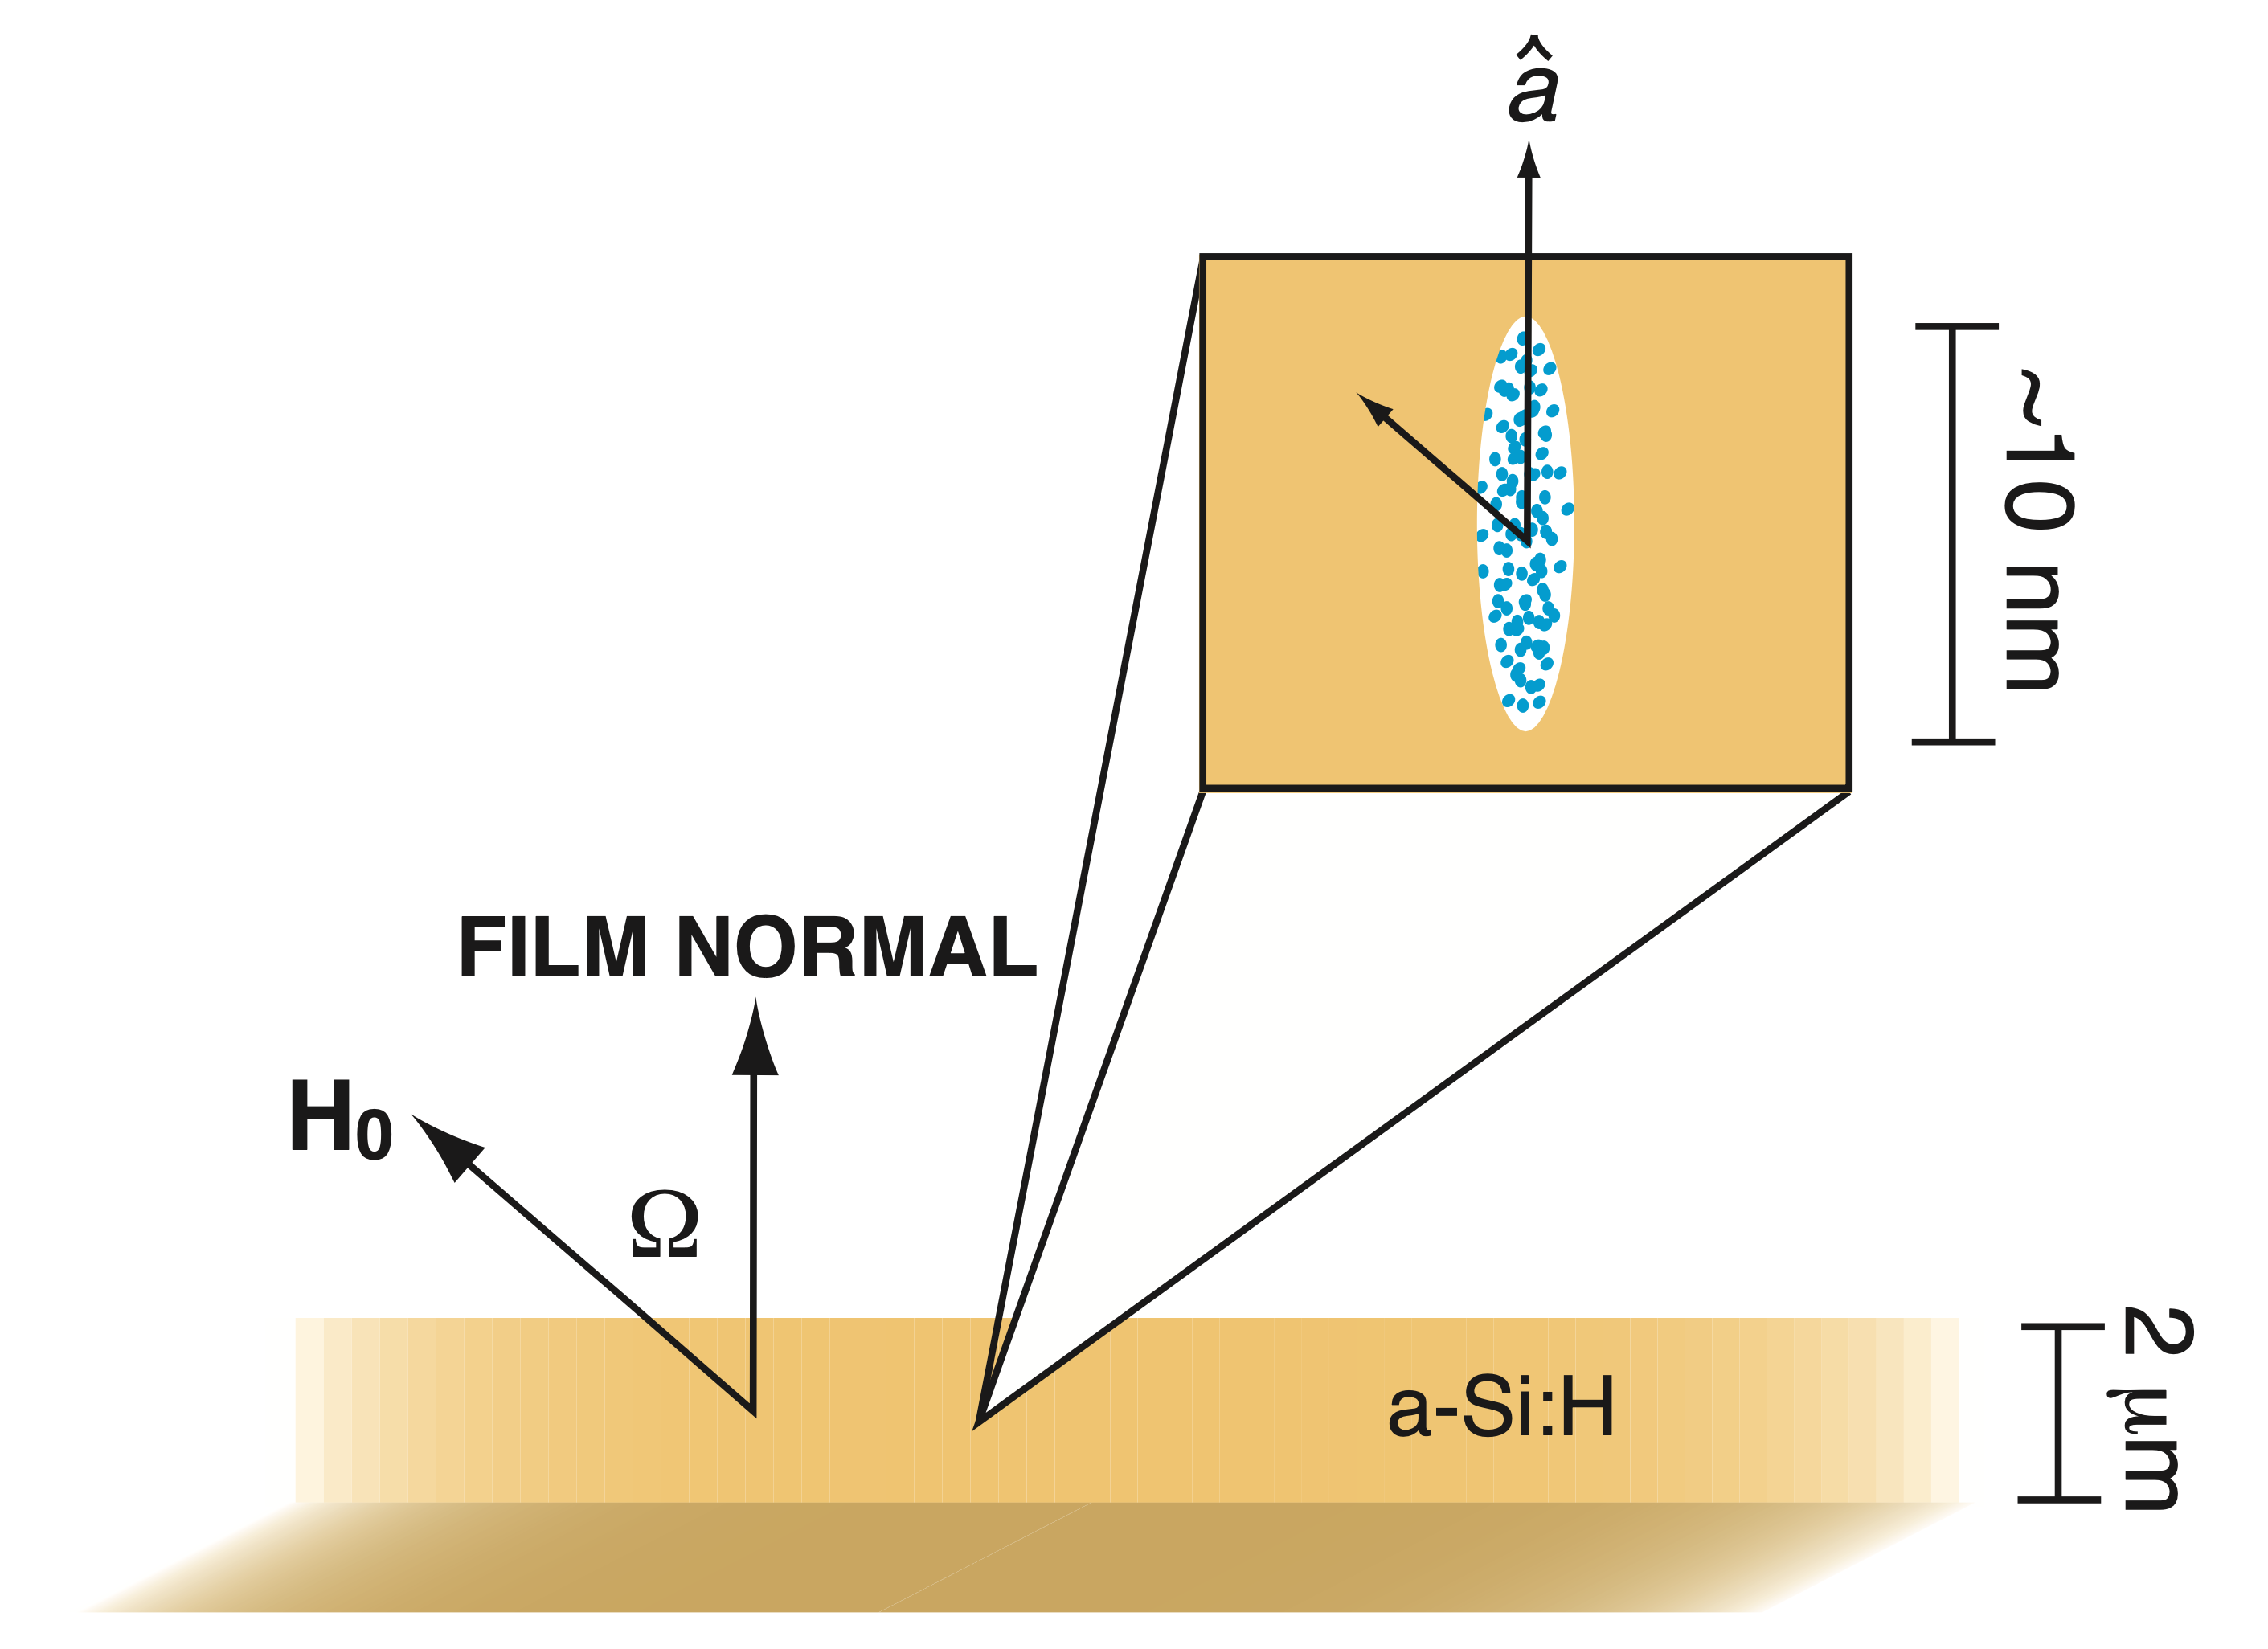
\includegraphics[width=\textwidth]{sample-nanopore-film.png}
      \caption{
        Значение константы связи $D$ зависит как от газа,
        так и от эффективного давления в нанопоре ($\approx 1$ кБар)
      }
    \end{subfigure}
    \captionsetup{skip=-0.1mm}
    \caption{}
  \end{figure}

  % \begin{block}{Нанопора\footnote[frame]{J. Baugh, A. Kleinhammes, D. Han, Q. Wang, and Y. Wu, Science 294, 1505 (2001).}, заполненая частицами со спином $1/2$}
  %     Так как молекулярная диффузия газа быстрее флип-флоп процессов,
  %     вся система характеризуется одной константой взаимодейсвия $D$.
%
  %     \vspace{\baselineskip}
%
  %     Значение константы связи $D$ зависит как от газа, так и от эффективного давления в нанопоре ($\approx 1$ кБар).
  % \end{block}
\end{frame}
\note{
    Hydrogenated amorphous silicon (Гидрогенизированный аморфный кремний)

    Для исследования многочастичной запутанности нам нужна модель,
    в которой почти все частицы взаимодействуют друг с другом,
    а также она должна поддаваться счету.
    Мы решили рассмотреть модель эквивалентных спинов.
    Такой модели соотвествует нанопора заполеннея спин несущими частицами.

    Такие нанопоры получаются выдавлием под давлением ~ 1 кБар  на специальной подложке.

    Необходимо подчеркнуть, что существуют некоторые ограничения для реализации описанной модели при исследовании нанопористых соединений с МК - ЯМР-методами. Например, модель предполагает, что все нанопоры имеют одинаковый объем и одинаковую "несферическую" форму.

    Молекулярная диффузия газа очень быстрая в сравнениидиподьных флип флом процессов
    Каждая частица успевает обойти всю нанопору пока пройдет флипфлоп
    Поэтому можно описать взаимодействие с одной константой

    Среднняя константа связи зависит как от газа, так и от эффективного давления в нанопоре

    При низких температурах диффузия побеждает?
    Какие частицы?
}

\begin{frame}{Диагонализация гамильтониана}
Многоквантовый гамильтониан
$$
H_\mathrm{MQ} = - \dfrac{D}{4} \left\{
    \left( I^{+} \right)^2 + \left( I^{-} \right)^2
\right\}
$$
коммутирует с проектором квадрата полного углового момента
$ \left[ H_\mathrm{MQ}, \hat I^2 \right] = 0 $.
Следовательно, в базисе собственных значений  $\hat I^2$ и $I_z$  гамильтониан имеет блочно-диагональный вид :
$$
H_\mathrm{MQ} = \mathrm{diag} \left\{
    H_\mathrm{MQ}^{N/2},
    H_\mathrm{MQ}^{N/2 - 1},
    \dots
    H_\mathrm{MQ}^{N/2 - [N/2]}
\right\},
$$
где каждый блок соответствует собственному значению полного углового момента.
\end{frame}
\note{
    Так как в нашей модели все констаны одинаковые, МК гамильтониан упрощается.
    Этот гамильтониан коммутирует ...слайд...
}
\begin{frame}{Эволюция информации Фишера (PRA-19)}
  \begin{figure}
    \begin{subfigure}[t]{0.3\textwidth}
      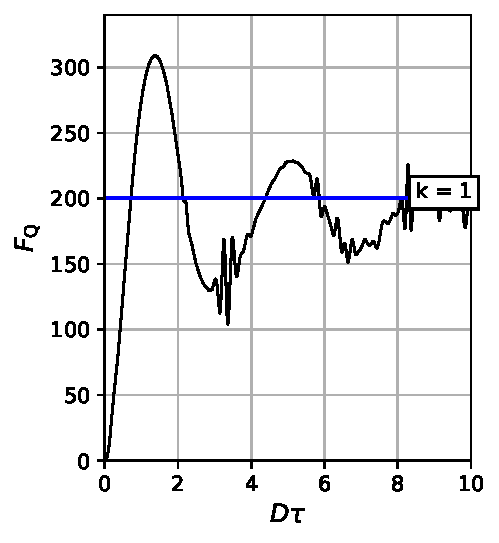
\includegraphics[width=\textwidth]{m2_t_b01.pdf}
      \caption{$\beta = 0.1$}
    \end{subfigure}
    \begin{subfigure}[t]{0.3\textwidth}
      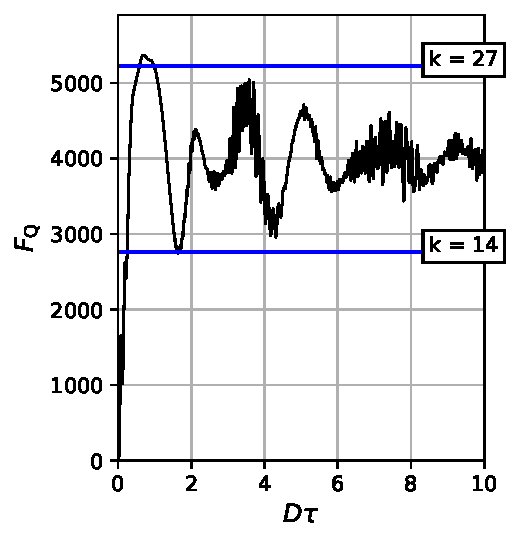
\includegraphics[width=\textwidth]{m2_t_b05.pdf}
      \caption{$\beta = 0.5$}
    \end{subfigure}
    \begin{subfigure}[t]{0.3\textwidth}
      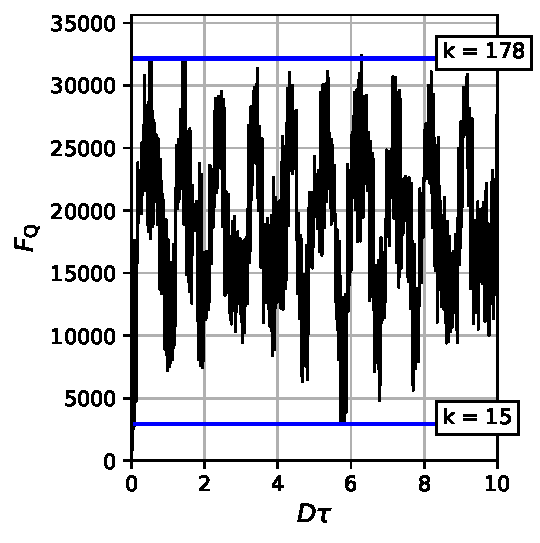
\includegraphics[width=\textwidth]{m2_t_b3_5.pdf}
      \caption{$\beta = 3.5$}
    \end{subfigure}
    \caption{Зависимость нижней границы информации Фишера от времени.}
  \end{figure}
\end{frame}


\begin{frame}{Температурная зависимость многочастичной запутанности (PRA-19)}
\begin{columns}
    \column{0.5\textwidth}
    \begin{figure}
    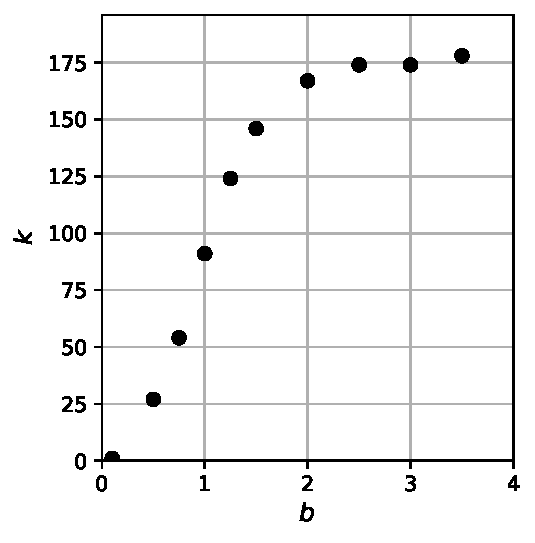
\includegraphics[width=0.7\textwidth]{k_b.pdf}
    \caption{Зависимость числа запутанных частиц от обратной температуры.}
    \end{figure}


    \column{0.5\textwidth}
    В начальный момент времени система находится в термодинамическом равновесии:
    $$
    \rho_\mathrm{eq} = \dfrac{ e^{\beta I_z} }{Tr \left\{ e^{\beta I_z} \right\} },
    \quad
    \beta = \dfrac{\hbar \omega_0}{k_{B} T}
    $$
\end{columns}
\end{frame}
\note{
При понижении температуры количество запутанных частиц стремительно растет.

При достаточно низкой температуре почти все спины запутаны друг с другом,
даже когда начальное состояние не было запутанно.

}


\begin{frame}{Дипольное упорядочение (JETP-20)\footnote{I.D. Lazarev and E.B. Fel'dman , \textit{JETP} \textbf{131}, 5, (2020)}}
  \alert{При дипольно упорядоченном начальном состоянии когерентности возникают быстрее.}
  $$
  \rho_i = \frac{1}{Z_i} e^\frac{\hslash\beta_\mathrm{d} \hdz}{k}
  \approx \frac{1}{Z_i}(1 + \frac{\hslash\beta_\mathrm{d}}{k} H_\mathrm{dz}),
  $$
  то есть зеемановская температура низкая, а дипольная --- высокая.
  \begin{block}{Методы создания дипольно упорядоченного состояния}
    \begin{itemize}
      \item  Адиабатическое размагничивание\footnote[frame]{C. P. Slichter and W. C. Holton, Phys. Rev. 122, 1701 (1961)} от большого значения приложенного поля до нуля во вращающейся системе координат.

      \item Двух-импульсный эксперимент Броекаерта-Джинира\footnote[frame]{J. Jeener and P. Broekaert, Phys. Rev. 157, 232 (1967).}.
  \end{itemize}
  \end{block}
\end{frame}
\note{

Был рассмотрен случай низкой зеемановской и высокой дипольной температурами, когда начальное состояние является

%Поэтому представляется целесообразным попытаться непосредственно охладить ядерную спиновую систему, используя то обстоятельство, что она относительно изолировапа от решетки из-за слабости механизмов спин-решеточной релаксации.

%Наиболее прямой метод охлаждения ядерных моментов заключается в их адиабатическом размагничивании от большого значепия приложенного поля до пуля. При обычных условиях охлаждение, получаемое этим способом, оказывается недостаточным.

%Например, адиабатическое размагничивание ядерной спиновой системы, выполняемое, скажем, при температуре решетки $Т_0 = 1$К, начиная с поля $H0 = 25 кЭ$, приводит к конечной температуре $T_f ~ T_0 H_L / H_0$, где величина локального поля $H_L$ состав­ляет несколько эрстед. В этом случае конечная темпера­тура будет порядка $10^{-4}$ К, что по крайней мере на два порядка превосходит требуемое зпачение.

Эксперимент Броекаерта-Джинира удобнее так как это естественные

Однако подходы, разработанные для этих исследований, ограничены случаем высоких температур и не могут применяться для изучения многоспиновой запутанности.

Но нам удалось теоретически доказать что двухимпульсная последовательность Брокаерта – Джинера [17, 19] позволяет получить дипольное упорядоченное состояние даже при низкой зеемановской температуре.

Также важно отметить, что гамильтониан Hdz частично усредняется быстрой молекулярной диффу- зией в нанопоре, а усредненный гамильтониан мож- но записать как
}

% \begin{frame}{Получение дипольно упорядоченого состояния}
% В начальный момент времени система находится в термодинамическом равновесии
% %
% $$
%     \rho(0) = \rho_\mathrm{eq} = \frac{1}{Z}
%     e^{
%       \frac{\hslash \omega_{0}}{k} \alpha_\mathrm{z} I_\mathrm{z}
%       + \frac{\hslash }{k} \beta_\mathrm{d} H_\mathrm{dz}
%     }
% $$
% %
% где $Z$ --- статистическая сумма; \\
% $\alpha_\mathrm{z}$, $\beta_\mathrm{d}$ --- обратные зеемановская и дипольная температуры; \\
% $H_\mathrm{dz}$ --- секулярная часть гамильтониана ДДВ в сильном внешнем магнитном поле;
% $$
%     H_\mathrm{dz} = \frac{D}{2} (3 I^{2}_{z} - I^{2})
% $$
% Нас интересует случай,
% когда зеемановская температура низкая, а дипольная --- высокая
% $$
%     \frac{\hslash \omega_{0}}{k} \alpha_\mathrm{z}\gg 1,
%     \quad\quad
%     \frac{\hslash D}{k}\beta_\mathrm{d} \ll 1
% $$
% \end{frame}
% \note{
%     В начальный момент времени ...
%     И мы уже рассмотрели этот случай в 19 году.
%     Однако в случае дипольного упорядочения когерентности...
%     А как я говорил, дисперсия распределеяня когерентностей связана с количеством запутанных частиц.
% }


\begin{frame}{Эволюция информации Фишера (JETP-20)}
  \begin{figure}
    \begin{subfigure}[t]{0.3\textwidth}
    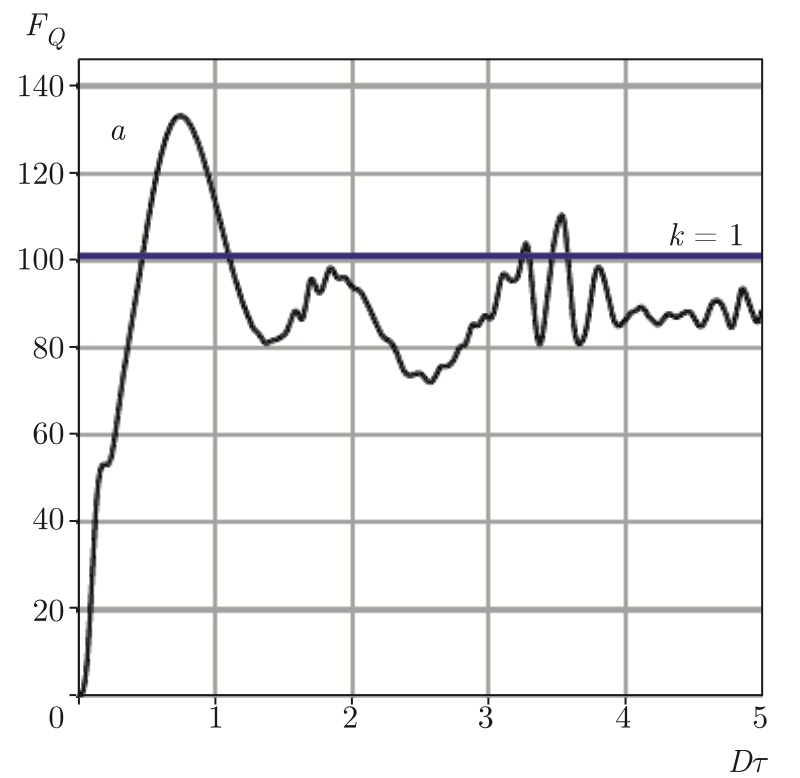
\includegraphics[width=\textwidth]{eval-1.png}
    \caption{$T = 6 \times 10^{-4}$ K}
    \end{subfigure}
    \hfill
    \begin{subfigure}[t]{0.3\textwidth}
      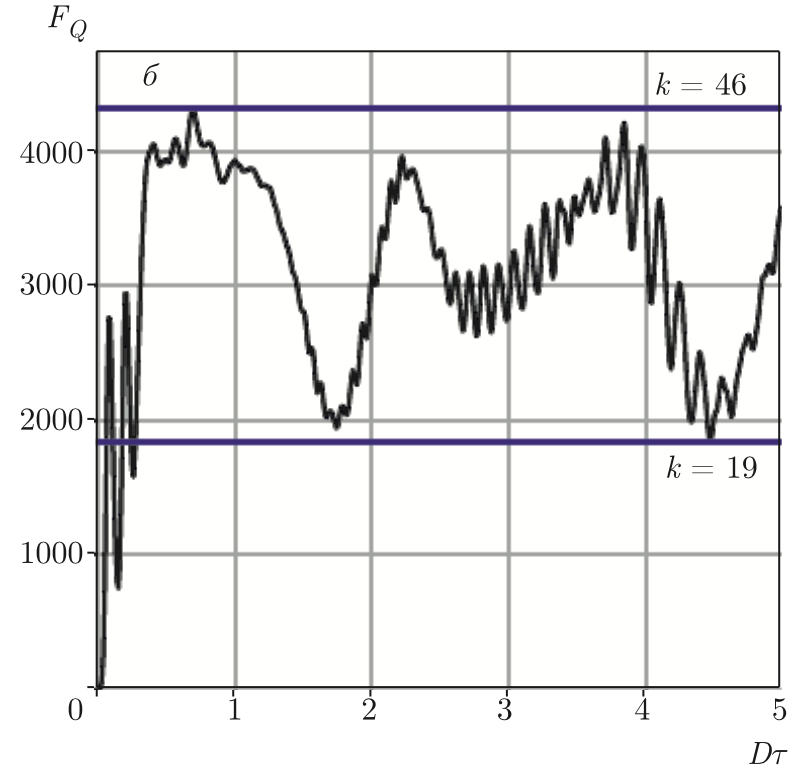
\includegraphics[width=\textwidth]{eval-2.png}
      \caption{$T = 3.2 \times 10^{-4}$ K}
    \end{subfigure}
    \hfill
    \begin{subfigure}[t]{0.3\textwidth}
      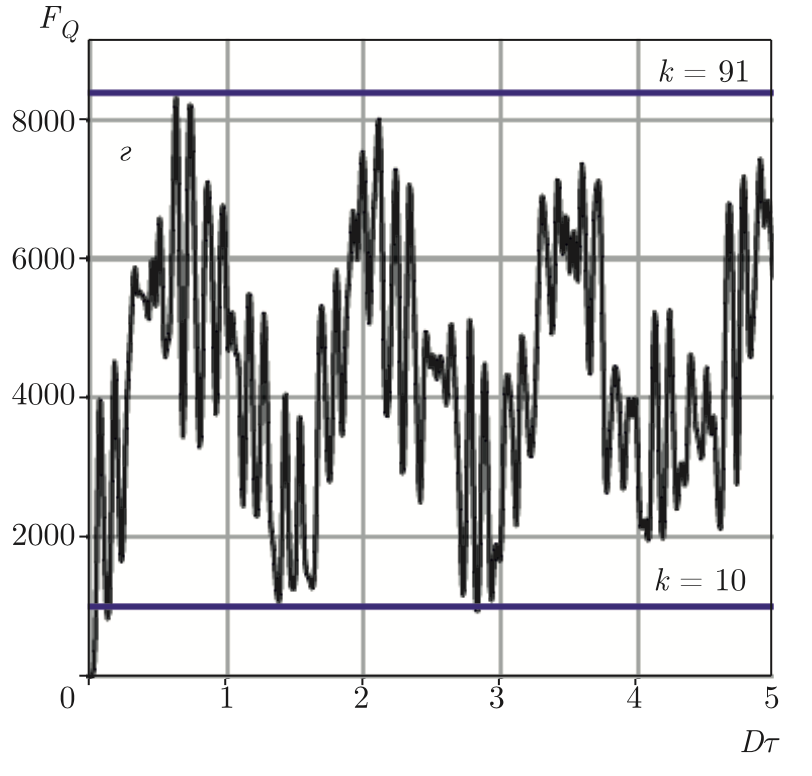
\includegraphics[width=\textwidth]{eval-3.png}
      \caption{$T = 4.8 \times 10^{-5}$ K}
    \end{subfigure}
    \caption{Зависимости нижней границы квантовой информации Фишера $F_Q = 2M_2$ от безразмерного времени $D\tau$ при $N = 101$.}
  \end{figure}
\end{frame}
\note{
    Нам удалось решить динамику для этой системы и изучить систему при разных значения температуры и размера системы.
}

\begin{frame}{Дипольное упорядочение (JETP-20)}
    \begin{figure}
    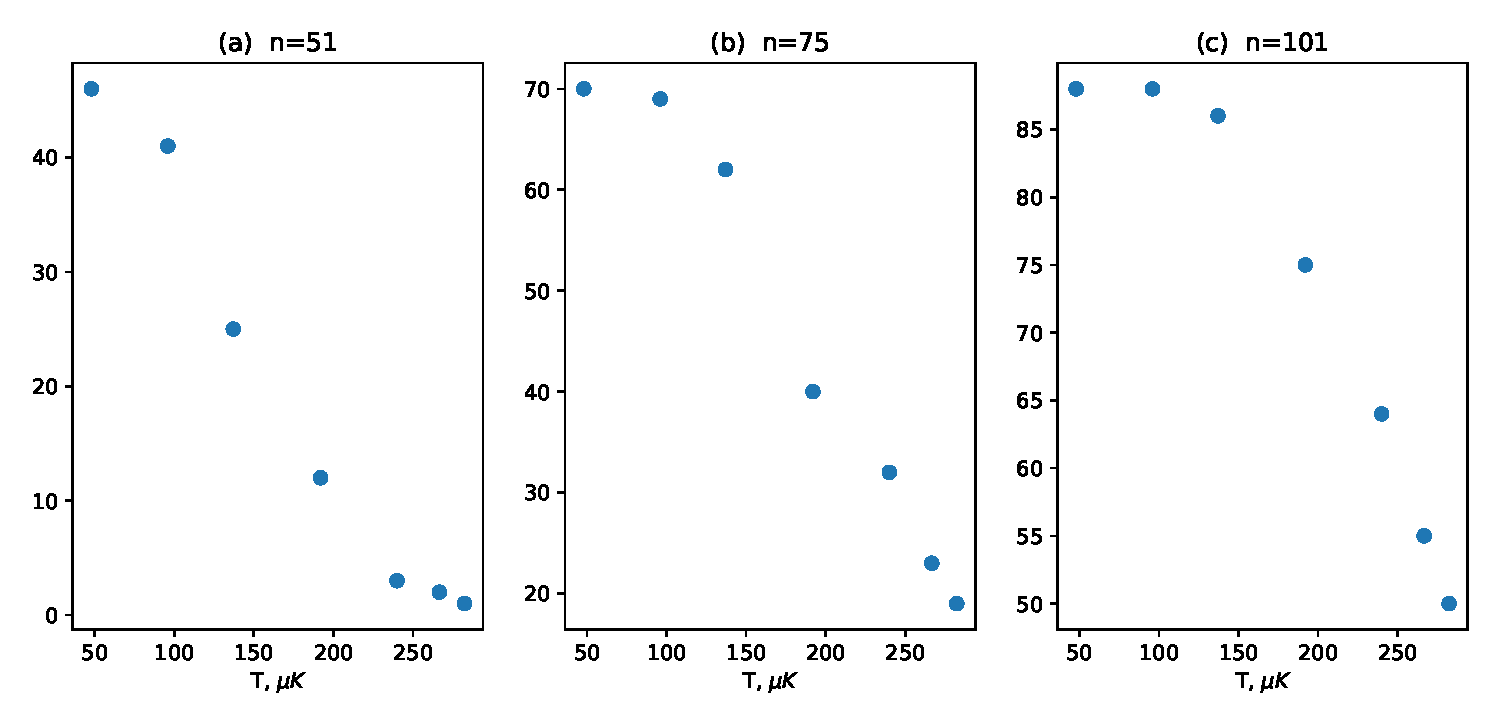
\includegraphics[width=0.7\textwidth]{entangled_spins_by_n.eps}
    \caption{Зависимости максимального количества числа запутанных частиц, усредненного по времени, эволюции от температуры.}
    \end{figure}
\end{frame}
\note{
мы хотели поймать скачак количества запутанных состояний, поэтому рассмотрели упорядочение

Максимальное количество запутанных спинов при одинаковой температуре увеличивается, когда увеличивается число спинов в нанопоре, потому что система в нанопоре становится плотнее.
}


\section{Многочастичная запутанность в квазиодномерных цепочках}
\begin{frame}{Однородная цепочка спинов}
  \begin{columns}
    \column{0.35\textwidth}
    \begin{figure}
      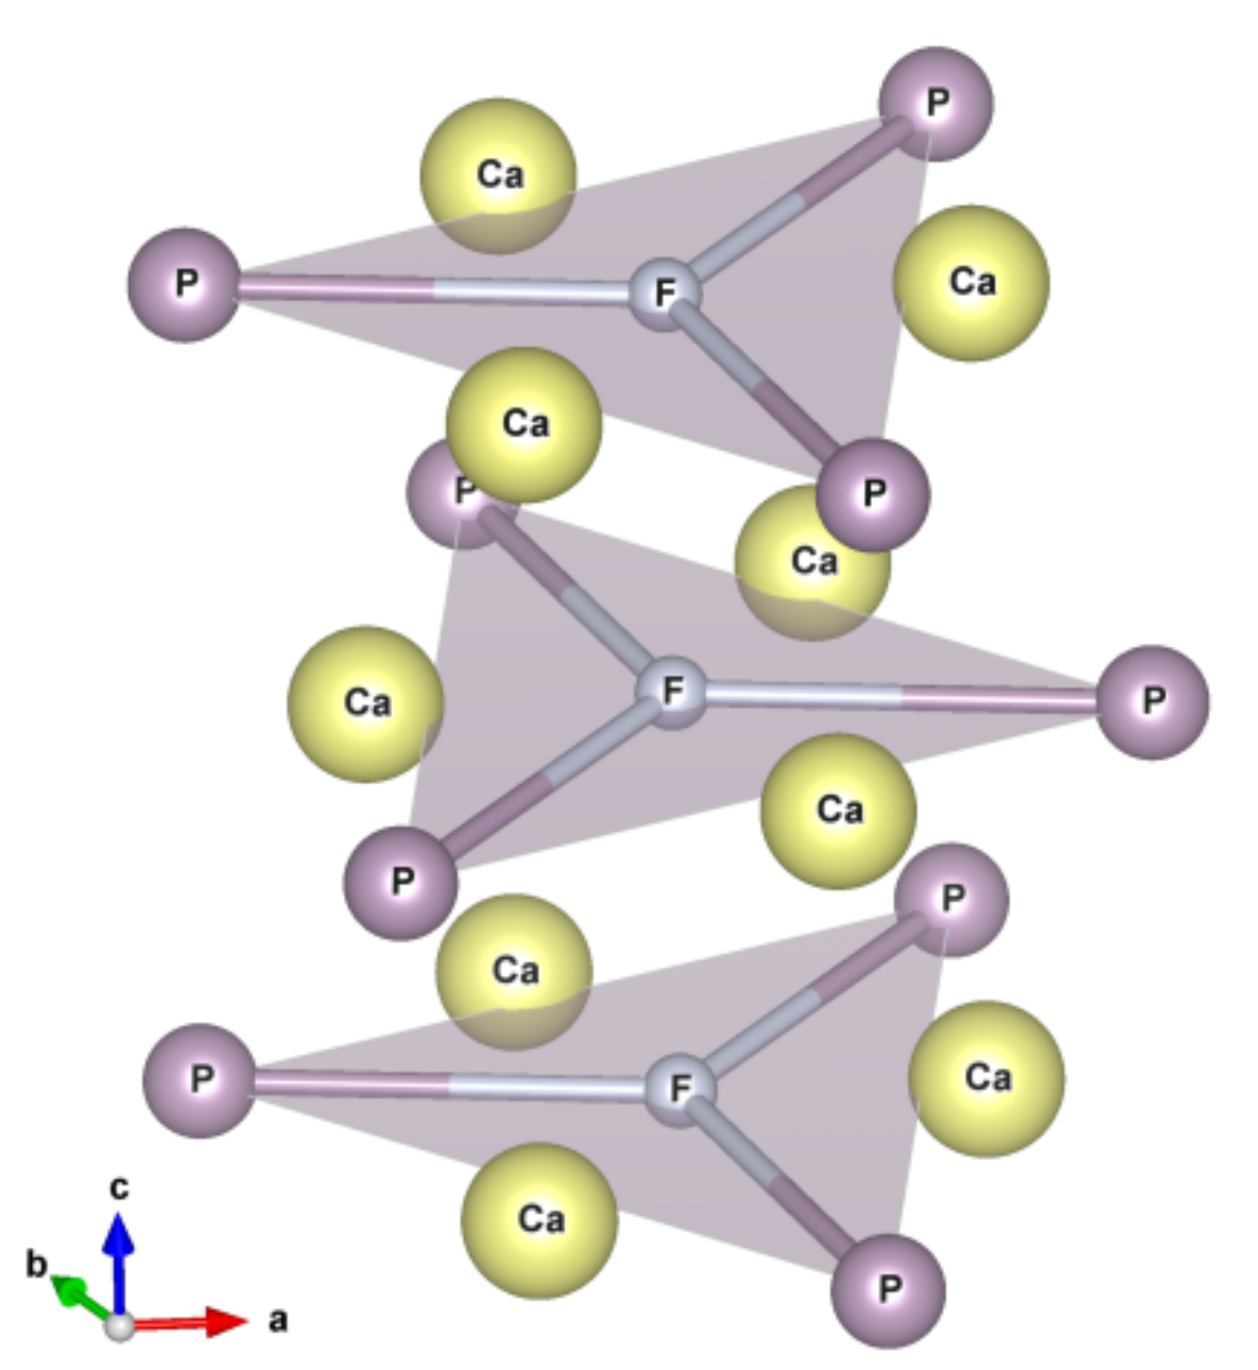
\includegraphics[width=\textwidth]{sample-fap-crystal-structure-part.png}
      \caption{Фтористый апатит Ca$_{10}$(PO$_4$)$_6$F$_2$}
    \end{figure}

    \column{0.6\textwidth}
      Часть кристаллической структуры FAp, показывающая окружение атомов фтора.
      Атомы кислорода были удалены для ясности.
      Атомы фтора равномерно разнесены ($r_{FF}= 3.44$\AA) и расположены в колонны вдоль $c$-оси кристалла.
      Каждый атом фтора окружен тремя равноудаленными атомами фосфора при $r_{FP} = 3.67$\AA,
      которые расположены в вершинах равносторонних треугольников на плоскости, перпендикулярной к $c$-оси,
      а также тремя ионами Ca\textrm{II} на расстоянии $2.34$\AA.
  \end{columns}
\end{frame}
\note{
  Фтористый апатит.
}

\begin{frame}{Альтернированная цепочка}
\begin{columns}

    \column{0.3\textwidth}
    \begin{figure}
    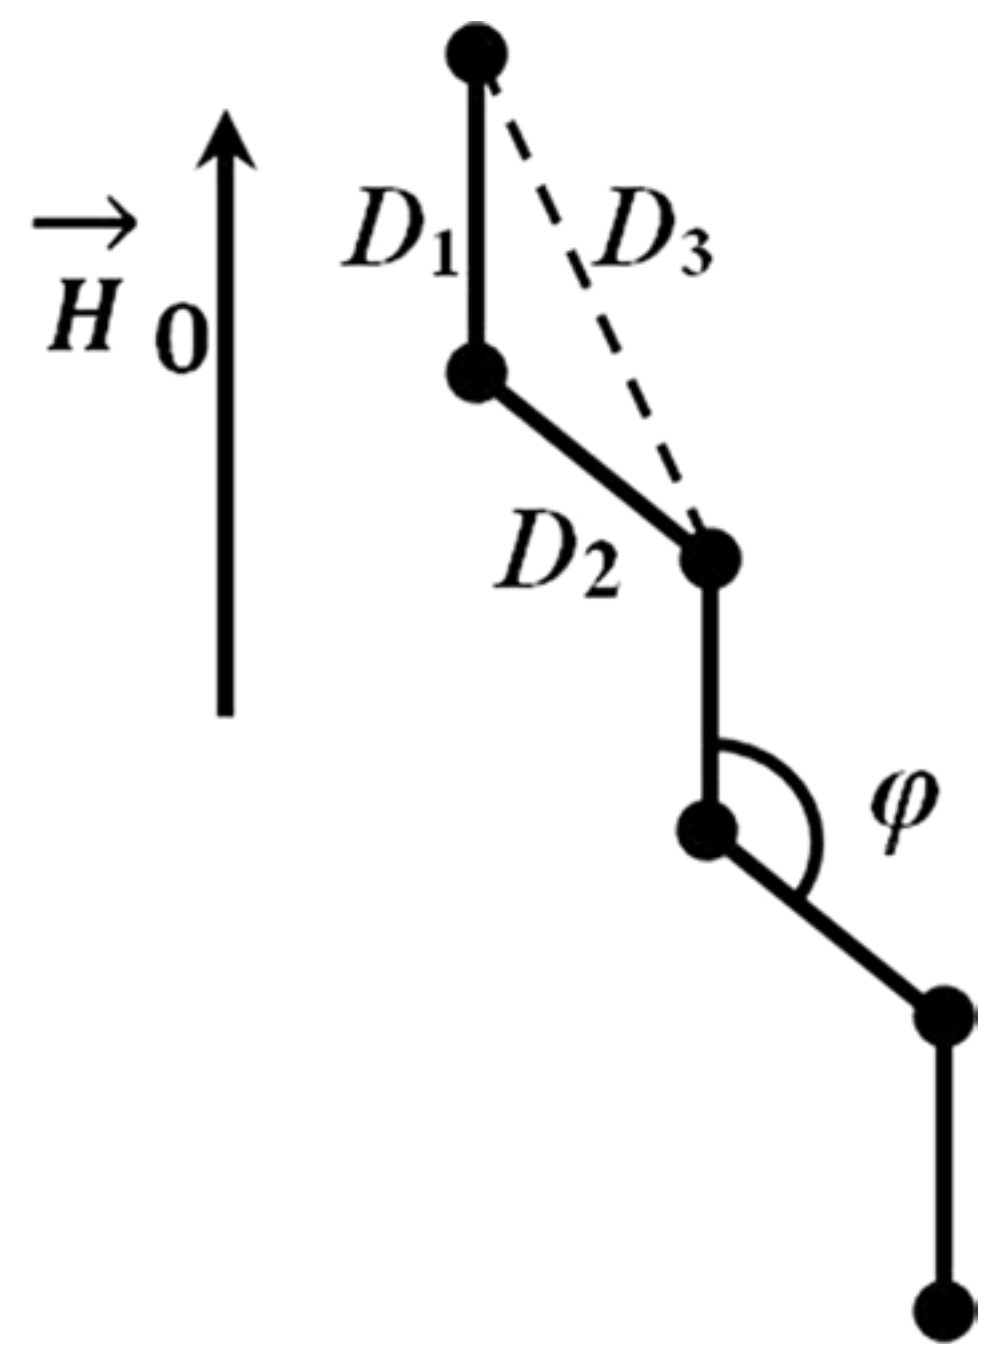
\includegraphics[width=1.0\textwidth]{model-zigzag-chain-schema.png}
    \caption{}
    \end{figure}

    \column{0.6\textwidth}
    \begin{block}{Константы взаимодействия}
        $$D_1=\dfrac{\gamma^2\hbar }{r^3}, $$
        $$D_2 = D_1\dfrac{ 3\cos^2 \varphi -1 }{2}, $$
        $$D_3 = D_1 \dfrac{ 3\sin^2 \frac{\varphi}{2} -1}{16 \sin^3, \frac{\varphi}{2}},$$
        где $\gamma$ - гиромагнитное отношение,
        $\varphi$ - угол между соседними связями,
        $r$ - расстояние между соседними спинами в цепочке.
    \end{block}

\end{columns}
\end{frame}
\note{
    Базовый случай это когда одна линия связи направлена вдоль поля. тогда констаты будет самой большой в доль поля.
    Изменяя угол к полю мы можем получить как альтернированную цепочку так и однородную.
    В приближении ближайших и следующих соседей, задача решается аналитически, но она
    не дает полной картины. Поэтому мы решали данную систему численно.
}

\begin{frame}{Альтернированная цепочка (JMR-20)\footnote[frame]{
        G.A. Bochkin and et al., \textit{J. Magn. Res.} \textbf{319}, 106816, (2020)}}
\begin{columns}

    \column{0.4\textwidth}
    \begin{figure}
      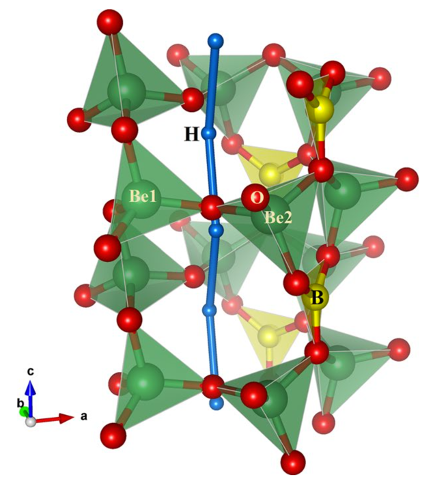
\includegraphics[width=0.85\textwidth]{model-zigzag-chain-hambergite-structure.png}
      \caption{}
    %\caption{Hанопора со спин-несущих молекулами во внешнем сильном магнитном поле $\vec B$}
    \end{figure}

    \column{0.6\textwidth}
    \begin{block}{Гамбергит $Be_2BO_3(OH)$ }
        \begin{itemize}
            \item Дипольное взаимодействие между ближайшими спинами протонов в цепи в 17 раз сильнее, чем со спинами окружающих цепей (в худшем случае).
            \item Взаимодействия с остальными окружающими спинами по меньшей мере в 30 раз слабее.
            \item Вклад дипольной связи между спинами в одной и той же цепи доминирует над остальными взаимодействиями.
        \end{itemize}
    \end{block}

\end{columns}
\end{frame}
\note{
    В одномерных цепочках возникают когерентности только $\pm 2$ порядка
    и следовательно дисперсия распределения будет небольшой
    и мы не увидим запутанных кластеров.
    Однако в альтернированная цепочке гамбергита возникают когерентности $\pm 4$ порядка
    и следовательно можно использовать эту модель для исследования многочастичной запутанности.
    The distance to these two protons is 4.49 Å
    The distance between a given chain and surrounding proton chains is at least 2.1 times larger than the distance between neighbors in the chain.

  % JMR 2020
}
\begin{frame}{Эволюция нижней границы информации Фишера (AMR-20)\footnote{G.A. Bochkin et al., \textit{Appl. Magn. Res.} \textbf{51}, 667-678, (2020)}}
\begin{columns}

    \column{0.6\textwidth}
    \begin{figure}
    \includegraphics[width=0.95\textwidth]{m2-by-time-in-zigzag-chain-with-n6-beta10.eps}
    %\caption{Hанопора со спин-несущих молекулами во внешнем сильном магнитном поле $\vec B$}
    \end{figure}

    \column{0.4\textwidth}
    Зависимость нижней границы квантовой информации Фишера
    $$ F_Q = 2M_2(\tau, T) $$
    от безразмерного времени $D_1 \tau$
    для шести спинов
    при температуре $T = 2.5 \times 10^{-3}$ $(b = 10)$.
    Область многочастичной запутанности ограничена горизонтальными линиями $k = 1$, $k = 5$.
\end{columns}
\end{frame}
\note{
   Мы не можем точно сказать сколько спинов запутанно,
   но можем дать нижнюю оценку на количество запутанных между собой спинов.
}


\begin{frame}{Максимальное количество запутанных спинов (AMR-20)}
\begin{columns}

    \column{0.5\textwidth}
    \begin{figure}
    \includegraphics[width=\textwidth]{nent-by-n-b10.eps}
    %\caption{Hанопора со спин-несущих молекулами во внешнем сильном магнитном поле $\vec B$}
    \end{figure}

    \column{0.5\textwidth}
    Зависимость максимального количества запутанных спинов $N_\mathrm{ent}$ от длины цепи при температуре $T = 2.5 \times 10^{-3}$ $(b = 10)$.

    \vspace{0.5cm}

    \alert{Создание запутанных кластеров в рассматриваемых зигзагообразных цепочках ограничено слабыми дипольными взаимодействиями удаленных спинов}.
\end{columns}
\end{frame}
\note{
  Установлено что, при фиксированной температуре с ростом числа спинов в цепи размер запутанных кластеров может уменьшаться;
}


\begin{frame}{Максимальное количество запутанных спинов (AMR-20)}
  \begin{columns}

     \column{0.6\textwidth}
     \begin{figure}
     \includegraphics[width=\textwidth]{nent-by-beta-n8-n6.eps}
     \end{figure}

     \column{0.4\textwidth}
     Зависимость максимального количества запутанных спинов $N_\mathrm{ent}$ от обратной температуры $b$
     $$ b=\dfrac{\hbar\omega_0}{kT} $$
     в зигзагообразной цепочки из 6 и 8 спинов.

  \end{columns}
\end{frame}
\note{
    Для 6 спинов накачка происходит быстрее, чем для 8 спинов.
}


\section{Измерение информации Вигнера-Янасе в МК эксперименте ЯМР}
\begin{frame}{Определения косой информации Вигнера-Янасе в МК ЯМР (PLA-21)\footnote{S.I. Doronin, E.B. Fel'dman,  I.D. Lazarev, \textit{Phys. Lett. A} \textbf{406}, 127458 (2021)}}
  \begin{block}{Термодинамически равновесное начальное состояние системы}
    \centering
    $
      \rho(0) = \rho_\mathrm{eq} = \frac{\exp(\frac{\hbar \omega_0}{kT}I_z)}{Z},
      \quad
      Z=Tr \left\{exp\left(\frac{\hbar \omega_0}{kT}I_z\right) \right\}
    $
  \end{block}

  Косая информация Вигнера-Янасе определяется как
  $$
  I_{WY}(\rho(\tau,\beta),I_z)
  = -2Tr([\sqrt{\rho(\tau,\beta)},I_z])^2,
  $$

  Эволюционная матрица плотности может быть представлена в виде
  $$
    \rho(\tau,\beta) = V^+(\tau) \frac{e^{\beta I_z}}{Z}V(\tau), \quad V(\tau) = e^{iH_{MQ}\tau}
  $$

  Используем взаимосвязь:
  $$
    \sqrt{\rho(\tau,\beta)} =
        \sqrt{V^+(\tau)\frac{e^{\beta I_z}}{Z}V(\tau)} =
            V^+(\tau) \frac{e^{\frac{\beta}{2}I_z}}{\sqrt{Z}}V(\tau).
  $$

\end{frame}
\note{
  We start with initial thermodynamic equilibrium density matrix.
  $\hbar$ and $k$ are the Plank and Boltzmann constants, respectively,
  $\omega_0$ is the Larmor frequency,
  $T$ is the temperature,
  and $I_z$ is the operator of the projection of the total spin angular momentum on the $z$-axis,
  which is directed along the strong external magnetic field.

  The Wigner–Yanase skew information is defined as presented.

  Now we use the evident relationship:

  And now we can see that this part a similar to the evolution density matrix at double temperature.
}

\begin{frame}{Определения косой информации Вигнера-Янасе в МК ЯМР (PLA-21)}
Получаем
%
$$
    \left[I_z,\sqrt{\rho(\tau,\beta)}\right]
    = \left[I_z, \sum_k \rho_k \left(\tau, \frac{\beta}{2}\right)\right]
    = \sum_k k\rho_k \left(\tau, \frac{\beta}{2}\right),
$$
%
и
%
$$
	Tr\left[I_z,\sqrt{\rho(\tau,\beta)} \right]^2
	= Tr\left\{\sum_{k,k'}kk'
		\rho_k\left(\tau,\frac{\beta}{2}\right)
		\rho_{k'}\left(\tau,\frac{\beta}{2}\right)
	\right\}
	= \sum_k k^2 J_k\left(\tau,\frac{\beta}{2}\right).
$$


\begin{alertblock}{}
\centering
$
  I_{WY}\left(\rho(\tau, \beta), I_z\right)
  = 2\sum_k k^2 J_k\left(\tau, \frac{\beta}{2}\right)
  = 2M_2\left(\tau, \frac{\beta}{2}\right)
$
\end{alertblock}

\end{frame}
\note{
  Then we have ... and ...
  Thus, we obtain an important observation.
  If the spin system is investigated with MQ NMR at the temperature $T \approx \beta^{−1}$
  then the Wigner–Yanase skew information equals to the double second moment
  of the distribution of the intensities of the MQ NMR coherences at the temperature $2T \approx 2\beta^{−1}$
  at any time during the spin evolution.
  The Wigner–Yanase skew information is connected with the second moment of the distribution
  of the MQ NMR coherences analogously to the Fisher information.
  Lets compare these informations.
}

\begin{frame}{Определения косой информации Вигнера-Янасе в МК ЯМР (PLA-21)}
  \begin{columns}
  \column{0.4\textwidth}
  %\vspace{-3mm}
  \begin{figure}
    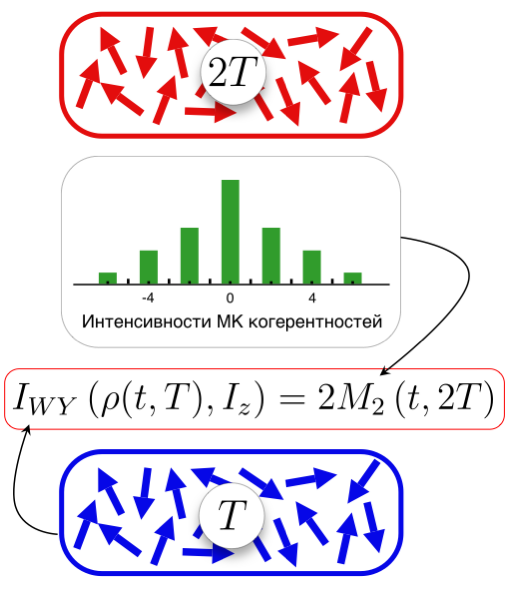
\includegraphics[width=0.9\textwidth]{wy-infromation-determination-cycle.png}
  \end{figure}
  \column{0.5\textwidth}
  Косая информация Вигнера-Янасе в системе с дипольным взаимодействием в МК эксперименте ЯМР при температуре T
  определяется\footnote[frame]{S. I. Doronin, E. B. Fel'dman,  I. D. Lazarev, \textit{Phys. Lett. A}, \textbf{406}, 127458 (2021)}
  удвоенным вторым моментом распределения МК когерентностей ЯМР при температуре 2T.
  \end{columns}
\end{frame}


\begin{frame}{Результаты: многочастичная запутанность (PLA-21)}
  \begin{columns}
    \column{0.5\textwidth}
    \begin{figure}
    \centering
    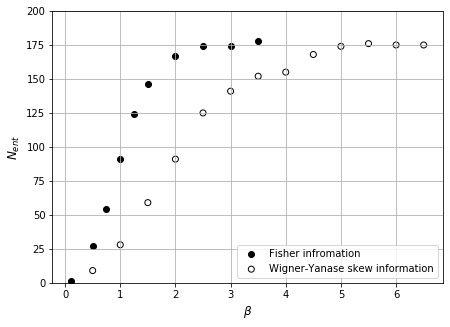
\includegraphics[width=0.9\textwidth]{nanopora_entangled_spins_by_temp}
    \caption{Зависимость числа запутанных частиц от обратной температуры $\beta=\frac{\hbar\omega_0}{kT}$.}
    \end{figure}


    \column{0.4\textwidth}
    \begin{block}{}
      \vspace{-2mm}
      $$
      I_{WY}\left(\rho(\tau, \beta), I_z\right)
      = 2M_2\left(\tau, \frac{\beta}{2}\right)
      $$

      $$
        F_Q\left(\rho(\tau, \beta)\right)
        \geq 2M_2\left(\tau, \beta \right)
      $$
      \vspace{0.1mm}
    \end{block}
    \begin{block}{}
      Связь косой информации Вигнера-Янасе и информации
      Фишера\footnote[frame]{S.Luo, Proc.Amer. Math.Soc. 132, No.885-890 (2003)}:
      $$
      I_{WY}\left(\rho, I_z\right)
      \leq I_F\left(\rho, I_z\right)
      \leq 2I_{WY}\left(\rho, I_z\right)
      $$
      \vspace{0.1mm}
    \end{block}
  \end{columns}
\end{frame}
\note{
  The restrictions allow us to hope that the obtained results for the number of the entangled spins are not very
  different.
  For the comparison we used the model~\cite{23} of a nonspherical nanopore filled with a gas of spin-carrying atoms
  (for example, xenon) or molecules in a strong external magnetic field.
  This model allows the investigation of the many-spin entanglement in the spin system consisting of hundreds of nuclear
  spins~\cite{8}.

  We investigated many-spin entanglement in the spin system, consisting of 201 spins, in a nanopore both with
  the Wigner--Yanase information $I_{WY}\left(\rho(\tau, \beta), I_z\right)$
  and the Fisher information $I_F\left(\rho(\tau,\beta),I_z\right)$.
  In Fig. the dependence of the number of the entangled spins on the inverse temperature is presented.
  black circles - the results are obtained with the Fisher information
  open circles - the results are obtained with the Wigner–Yanase information.
  Fig.~\ref{fig:2} demonstrates that the number of the entangled spins increases when the temperature decreases both for
  the Wigner--Yanase information and the Fisher information.
}

% \section{Многоквантовая динамика при низких температурах}
% \input{slides/results/mq-dynamic-at-low-temperature}
%
% \section{Многоспиновая запутанность в системе эквивалентных спинов}
% \input{slides/models/equivalent-spins}
% \input{slides/results/equivalent-spins-entanglement-with-term-equilibrium-state}
% \input{slides/results/equivalent-spins-entanglement-with-dipolar-ordered-state}
%
% \section{Многоспиновая запутанность в цепочках}
% \input{slides/models/zigzag-spin-chain}
% \input{slides/results/zigzag-spin-chain-entanglement}
%
% \section{Определение информации Вигнера-Янасе в МК эксперименте ЯМР}
% \input{slides/results/determination-of-wigner-yanase-information}
%
% \section{Сравнение информации Вигнера-Янасе и Фишера}
% \input{slides/results/comparison-wyi-and-fi}

\section{Итоги}
\begin{frame}{Положения, выносимые на защиту}
  \begin{enumerate}
  \item
  Разработанная теория МК ЯМР позволяет исследовать многочастичную запутанность в системе ядерных спинов при произвольной температуре.

  \item
  С понижением температуры количество запутанных спинов растет и в нанопоре, и в зигзагобразной цепочке. 
  % В нанопоре, заполненой спин несущими частицами, при температуре 
  % $T = 6.856\cdot10^{-3}$~K $(\beta=3.5)$ 
  % почти все спины (до 179 из 201) запутаны.
  %Исследована температурная зависимость многочастичной запутанности в нанопоре,
  %когда система приготовлена в термодинамическом равновесном зеемановском и дипольном упорядоченном состояниях.

  \item
  Оценка количества запутанных спинов в однородных цепочках согласуется с результатами, представленными в литературе.
  % Исследована многочастичная запутанность в квазиодномерных цепочках ядерных спинов в зависимости от параметров цепи и температуры.

  \item
  Если спиновая система исследуется в МК эксперименте ЯМР с начальным равновесным термодинамическим состоянием при температуре $T$, 
  то ее косая информация Вигнера-Янасе равна удвоенному второму моменту распределения интенсивностей МК когерентностей ЯМР системы, приготовленной при вдвое большей температуре $2T$ в тот же момент времени эволюции;
  % Предложен метод экспериментального измерения точного значения косой информации Вигнера-Янасе в рамках МК спектроскопии ЯМР.

  \item
  Результаты оценки количества запутанных спинов, полученные на основе квантовой информации Фишера и косой информации Вигнера-Янасе, согласуются;
  % Проведено сравнение оценок многочастичной запутанности, 
  % полученных на основе квантовой информации Фишера и косой информации Вигнера-Янасе.
\end{enumerate}

\end{frame}

\begin{frame}{Публикации}
  \begin{thebibliography}{}
    \bibitem{Doronin2019} S. I. Doronin, E. B. Fel'dman,  I. D. Lazarev, \textit{Physical Review A}, \textbf{100}, 022330 (2019)
\bibitem{Lazarev2020} I. D. Lazarev and E. B. Fel'dman , \textit{JETP}, \textbf{131}, 5, (2020)
\bibitem{Bochkin2020a} G.A. Bochkin, E.B. Fel'dman, E.I. Kuznetsova, I.D. Lazarev, S.G. Vasil'ev, V.I. Volkov, \textit{Journal of Magnetic Resonance}, \textbf{319}, 106816, (2020)
\bibitem{Bochkin2020b} G. A. Bochkin, S. I. Doronin, E. I. Kuznetsova, I. D. Lazarev, E. B. Fel’dman, S. G. Vasil’Ev, \textit{Applied Magnetic Resonance}, \textbf{51}, 667-678, (2020);
\bibitem{Doronin2021} S. I. Doronin, E. B. Fel'dman,  I. D. Lazarev, \textit{Physics Letters A}, \textbf{406}, 127458 (2021)
  \end{thebibliography}
\end{frame}

\begin{frame}{Благодарности}
  И.Д. Лазарев выражает благодарность научному руководителю Э.Б. Фельдману и коллегам Г.А. Бочкину, С.Г. Васильеву, С.И. Доронину, Е.И. Кузнецовой, А.H. Пыркову и А.И. Зенчуку.

И.Д. Лазарев выражает признательность за поддержку Фонду развития теоретической физики и математики ``Базис'' (№19-1-5-130-1).

Работа выполнена при поддержке фонда Министерства Науки и Высшего Образования Российской Федерации (№075-15- 2020-779) и частично (№075-15-2020-788).
\end{frame}

% \input{slides/suplemental-materials}

\end{document}
